% Options for packages loaded elsewhere
\PassOptionsToPackage{unicode}{hyperref}
\PassOptionsToPackage{hyphens}{url}
\PassOptionsToPackage{dvipsnames,svgnames,x11names}{xcolor}
\documentclass[
  10pt,
  twocolumn,
  10pt]{article}
\usepackage{xcolor}
\usepackage[a4paper, margin=0.7in, columnsep=18pt]{geometry}
\usepackage{amsmath,amssymb}
\setcounter{secnumdepth}{-\maxdimen} % remove section numbering
\usepackage{iftex}
\ifPDFTeX
  \usepackage[T1]{fontenc}
  \usepackage[utf8]{inputenc}
  \usepackage{textcomp} % provide euro and other symbols
\else % if luatex or xetex
  \usepackage{unicode-math} % this also loads fontspec
  \defaultfontfeatures{Scale=MatchLowercase}
  \defaultfontfeatures[\rmfamily]{Ligatures=TeX,Scale=1}
\fi
\usepackage{lmodern}
\ifPDFTeX\else
  % xetex/luatex font selection
\fi
% Use upquote if available, for straight quotes in verbatim environments
\IfFileExists{upquote.sty}{\usepackage{upquote}}{}
\IfFileExists{microtype.sty}{% use microtype if available
  \usepackage[]{microtype}
  \UseMicrotypeSet[protrusion]{basicmath} % disable protrusion for tt fonts
}{}
\makeatletter
\@ifundefined{KOMAClassName}{% if non-KOMA class
  \IfFileExists{parskip.sty}{%
    \usepackage{parskip}
  }{% else
    \setlength{\parindent}{0pt}
    \setlength{\parskip}{6pt plus 2pt minus 1pt}}
}{% if KOMA class
  \KOMAoptions{parskip=half}}
\makeatother
\usepackage{color}
\usepackage{fancyvrb}
\newcommand{\VerbBar}{|}
\newcommand{\VERB}{\Verb[commandchars=\\\{\}]}
\DefineVerbatimEnvironment{Highlighting}{Verbatim}{commandchars=\\\{\}}
% Add ',fontsize=\small' for more characters per line
\usepackage{framed}
\definecolor{shadecolor}{RGB}{248,248,248}
\newenvironment{Shaded}{\begin{snugshade}}{\end{snugshade}}
\newcommand{\AlertTok}[1]{\textcolor[rgb]{0.94,0.16,0.16}{#1}}
\newcommand{\AnnotationTok}[1]{\textcolor[rgb]{0.56,0.35,0.01}{\textbf{\textit{#1}}}}
\newcommand{\AttributeTok}[1]{\textcolor[rgb]{0.13,0.29,0.53}{#1}}
\newcommand{\BaseNTok}[1]{\textcolor[rgb]{0.00,0.00,0.81}{#1}}
\newcommand{\BuiltInTok}[1]{#1}
\newcommand{\CharTok}[1]{\textcolor[rgb]{0.31,0.60,0.02}{#1}}
\newcommand{\CommentTok}[1]{\textcolor[rgb]{0.56,0.35,0.01}{\textit{#1}}}
\newcommand{\CommentVarTok}[1]{\textcolor[rgb]{0.56,0.35,0.01}{\textbf{\textit{#1}}}}
\newcommand{\ConstantTok}[1]{\textcolor[rgb]{0.56,0.35,0.01}{#1}}
\newcommand{\ControlFlowTok}[1]{\textcolor[rgb]{0.13,0.29,0.53}{\textbf{#1}}}
\newcommand{\DataTypeTok}[1]{\textcolor[rgb]{0.13,0.29,0.53}{#1}}
\newcommand{\DecValTok}[1]{\textcolor[rgb]{0.00,0.00,0.81}{#1}}
\newcommand{\DocumentationTok}[1]{\textcolor[rgb]{0.56,0.35,0.01}{\textbf{\textit{#1}}}}
\newcommand{\ErrorTok}[1]{\textcolor[rgb]{0.64,0.00,0.00}{\textbf{#1}}}
\newcommand{\ExtensionTok}[1]{#1}
\newcommand{\FloatTok}[1]{\textcolor[rgb]{0.00,0.00,0.81}{#1}}
\newcommand{\FunctionTok}[1]{\textcolor[rgb]{0.13,0.29,0.53}{\textbf{#1}}}
\newcommand{\ImportTok}[1]{#1}
\newcommand{\InformationTok}[1]{\textcolor[rgb]{0.56,0.35,0.01}{\textbf{\textit{#1}}}}
\newcommand{\KeywordTok}[1]{\textcolor[rgb]{0.13,0.29,0.53}{\textbf{#1}}}
\newcommand{\NormalTok}[1]{#1}
\newcommand{\OperatorTok}[1]{\textcolor[rgb]{0.81,0.36,0.00}{\textbf{#1}}}
\newcommand{\OtherTok}[1]{\textcolor[rgb]{0.56,0.35,0.01}{#1}}
\newcommand{\PreprocessorTok}[1]{\textcolor[rgb]{0.56,0.35,0.01}{\textit{#1}}}
\newcommand{\RegionMarkerTok}[1]{#1}
\newcommand{\SpecialCharTok}[1]{\textcolor[rgb]{0.81,0.36,0.00}{\textbf{#1}}}
\newcommand{\SpecialStringTok}[1]{\textcolor[rgb]{0.31,0.60,0.02}{#1}}
\newcommand{\StringTok}[1]{\textcolor[rgb]{0.31,0.60,0.02}{#1}}
\newcommand{\VariableTok}[1]{\textcolor[rgb]{0.00,0.00,0.00}{#1}}
\newcommand{\VerbatimStringTok}[1]{\textcolor[rgb]{0.31,0.60,0.02}{#1}}
\newcommand{\WarningTok}[1]{\textcolor[rgb]{0.56,0.35,0.01}{\textbf{\textit{#1}}}}
\usepackage{longtable,booktabs,array}
\newcounter{none} % for unnumbered tables
\usepackage{calc} % for calculating minipage widths
% Correct order of tables after \paragraph or \subparagraph
\usepackage{etoolbox}
\makeatletter
\patchcmd\longtable{\par}{\if@noskipsec\mbox{}\fi\par}{}{}
\makeatother
% Allow footnotes in longtable head/foot
\IfFileExists{footnotehyper.sty}{\usepackage{footnotehyper}}{\usepackage{footnote}}
\makesavenoteenv{longtable}
\usepackage{graphicx}
\makeatletter
\newsavebox\pandoc@box
\newcommand*\pandocbounded[1]{% scales image to fit in text height/width
  \sbox\pandoc@box{#1}%
  \Gscale@div\@tempa{\textheight}{\dimexpr\ht\pandoc@box+\dp\pandoc@box\relax}%
  \Gscale@div\@tempb{\linewidth}{\wd\pandoc@box}%
  \ifdim\@tempb\p@<\@tempa\p@\let\@tempa\@tempb\fi% select the smaller of both
  \ifdim\@tempa\p@<\p@\scalebox{\@tempa}{\usebox\pandoc@box}%
  \else\usebox{\pandoc@box}%
  \fi%
}
% Set default figure placement to htbp
\def\fps@figure{htbp}
\makeatother
\setlength{\emergencystretch}{3em} % prevent overfull lines
\providecommand{\tightlist}{%
  \setlength{\itemsep}{0pt}\setlength{\parskip}{0pt}}
\usepackage{float}
\usepackage{graphicx}
\usepackage{booktabs}
\usepackage[font=small,labelfont=bf]{caption}
\usepackage{titlesec}
\titleformat*{\section}{\normalsize\bfseries}
\titleformat*{\subsection}{\small\bfseries}
\titlespacing*{\section}{0pt}{6pt}{2pt}
\titlespacing*{\subsection}{0pt}{4pt}{1pt}
\setlength{\parskip}{2pt}
\setlength{\parindent}{0pt}
\setlength{\textfloatsep}{6pt}
\setlength{\intextsep}{6pt}
\widowpenalty=10000
\clubpenalty=10000
\usepackage{bookmark}
\IfFileExists{xurl.sty}{\usepackage{xurl}}{} % add URL line breaks if available
\urlstyle{same}
\hypersetup{
  pdftitle={Predicting Spatial Query Selectivity on Chicago Crime Data},
  pdfauthor={Rahul Sanjay Mandviya · Manthan Surjuse · Atharva Patil · Prasanna Renapurkar},
  colorlinks=true,
  linkcolor={black},
  filecolor={Maroon},
  citecolor={Blue},
  urlcolor={blue},
  pdfcreator={LaTeX via pandoc}}

\title{Predicting Spatial Query Selectivity on Chicago Crime Data}
\usepackage{etoolbox}
\makeatletter
\providecommand{\subtitle}[1]{% add subtitle to \maketitle
  \apptocmd{\@title}{\par {\large #1 \par}}{}{}
}
\makeatother
\subtitle{CSP 571 --- UCI Dataset \#493 Query Analytics Workloads}
\author{Rahul Sanjay Mandviya · Manthan Surjuse · Atharva Patil ·
Prasanna Renapurkar}
\date{May 2026}

\begin{document}
\maketitle

\section{Section 1 --- Abstract}\label{section-1-abstract}

Spatial query selectivity estimation --- predicting how many records a
range or radius query will touch --- is a foundational problem in
database query optimisation. We study UCI Machine Learning Repository
dataset \#493 (Anagnostopoulos and Triantafillou 2015), comprising
260,000 synthetic spatial queries (200,000 range + 60,000 radius) over
the City of Chicago crime database, and pose two regression tasks:
predicting the number of records returned (\texttt{Count}) and their sum
(\texttt{SUM}) for each query.

After de-duplicating, schema-validating, and feature-engineering the raw
data (157 structural nulls imputed; per-file coordinate normalisation;
spatial features including \texttt{area}, \texttt{dist\_centroid}, and a
boundary-crossing flag), we compare four model families --- Linear
Regression, Random Forest (500 trees), XGBoost (5-fold CV grid search),
and KNN (K ∈ \{5, 10, 20\}) --- on an 80/20 train--test split (seed =
42). XGBoost wins on both sub-datasets: Range test RMSE = 6,575 (R² =
0.998), Radius test RMSE = 8.52 (R² = 0.996), reducing the
linear-baseline RMSE by 88.9\% and 92.2\% respectively. K-Means
clustering and per-decile residual analysis identify large-area and
city-edge queries as the dominant residual-risk segment. Future work:
extended boosting (the \texttt{nrounds} cap was hit), a boundary-aware
Radius model, and a deep-learning baseline.

\section{Section 2 --- Overview}\label{section-2-overview}

\subsection{2.1 Problem Statement}\label{problem-statement}

Modern relational and spatial database engines rely on
\textbf{selectivity estimation} --- predicting the result-set size of a
query before execution --- to choose efficient query plans (Kipf et
al.~2019). Cardinality misestimation is the single largest source of
query-optimiser regression in production systems. UCI dataset \#493
(Anagnostopoulos and Triantafillou 2015) provides a controlled benchmark
for this task: 260,000 synthetic spatial queries against the City of
Chicago crime database, paired with ground-truth aggregates. The
supervised regression targets are \texttt{Count} (number of records
intersected) and \texttt{SUM} (sum of an aggregate field over the
records). A model that accurately maps query geometry → result size
could be embedded in a query planner as a learned cardinality estimator.

\subsection{2.2 Relevant Literature}\label{relevant-literature}

Tree-based ensembles have been the workhorses of tabular-data regression
for the past two decades. Random Forest (Breiman 2001) reduces variance
through bagging and feature subsampling but tends to memorise training
data on dense regression tasks. Gradient-boosted trees, and in
particular XGBoost (Chen and Guestrin 2016), introduce regularised
boosting with second-order optimisation and have repeatedly topped
public regression benchmarks. For spatial cardinality estimation
specifically, recent learned-database work (Kipf et al.~2019) has
demonstrated that gradient-boosted trees on hand-crafted geometric
features can match or exceed deep-learning estimators while remaining
order-of-magnitude cheaper to train and serve.

\subsection{2.3 Proposed Methodology}\label{proposed-methodology}

Our approach is a four-stage pipeline executed as a one-person-at-a-time
team sprint: (1) \textbf{data engineering} --- schema validation,
de-duplication, coordinate normalisation per file, and log-transform of
skewed targets; (2) \textbf{exploratory data analysis} ---
distributional and spatial visualisation, correlation/Spearman
screening, identification of multicollinearity (\texttt{area} vs
\texttt{X\_range\ ×\ Y\_range}); (3) \textbf{modeling} --- feature
engineering (\texttt{log\_area}, \texttt{aspect\_ratio},
\texttt{interact\_area\_dist}, \texttt{boundary\_flag}), VIF-based
feature selection for the linear baseline, and grid-search--tuned
XGBoost with 5-fold cross-validation; (4) \textbf{validation} ---
held-out-set diagnostics (residuals, predicted-vs-actual), unsupervised
K-Means clustering for spatial bias analysis, and per-decile/per-cluster
bias decomposition. All code is reproducible with seed = 42; the
pipeline runs end-to-end in R (no Python dependencies).

\section{Section 3 --- Data Processing}\label{section-3-data-processing}

\emph{Draft for the final report. \textasciitilde250 words. Owner:
Rahul. Handed off to Prasanna for integration.}

The Query Analytics Workloads dataset (UCI ML Repository \#493) ships as
three sub-files derived from Chicago crime records:
\texttt{Range-Queries-Aggregates} (200,000 rectangular range queries
with \texttt{Count}, \texttt{SUM}, and \texttt{AVG} targets),
\texttt{Radius-Queries} (50,000 disc queries with only geometric
parameters), and \texttt{Radius-Queries-Count} (10,000 disc queries with
a \texttt{Count} target). Every row was parsed in R with \texttt{readr},
and observed row counts exactly matched the totals reported on the UCI
page (260,000 combined). The full pipeline is reproducible from
\texttt{src/preprocess.R} and narrated in
\texttt{notebooks/01\_preprocessing.Rmd}.

Schema validation surfaced one anomaly the UCI card does not document:
157 rows in \texttt{Range-Queries-Aggregates} have \texttt{AVG\ =\ NA}
because \texttt{Count\ =\ 0} and \texttt{SUM\ =\ 0} make the ratio
undefined. These are structural zeros rather than data quality failures,
so \texttt{AVG} was imputed to 0 for those rows; no other nulls existed
in any file. Exact-duplicate detection removed zero rows across all
three files (100 \% retention). A boundary-effect check flagged queries
whose coverage extends past the per-dataset bounding box: 1,373 of the
200,000 range queries and effectively all radius queries --- a direct
consequence of the Gaussian sampling used to synthesize the workloads.

Feature engineering added four spatial features per row: \texttt{area}
(4·X\_range·Y\_range for rectangles; π·R² for discs), per-dataset
min-max-normalized \texttt{X\_norm} and \texttt{Y\_norm} ∈ {[}0, 1{]},
and \texttt{dist\_centroid} --- Euclidean distance from each query
center to the dataset mean. Because \texttt{Count} and \texttt{SUM} are
heavily right-skewed (skew \textgreater{} 3), \texttt{log1p} transforms
of both targets were exported alongside the raw variants so Day 3 can
model on whichever scale gives the best residuals.

\begin{figure}[H]
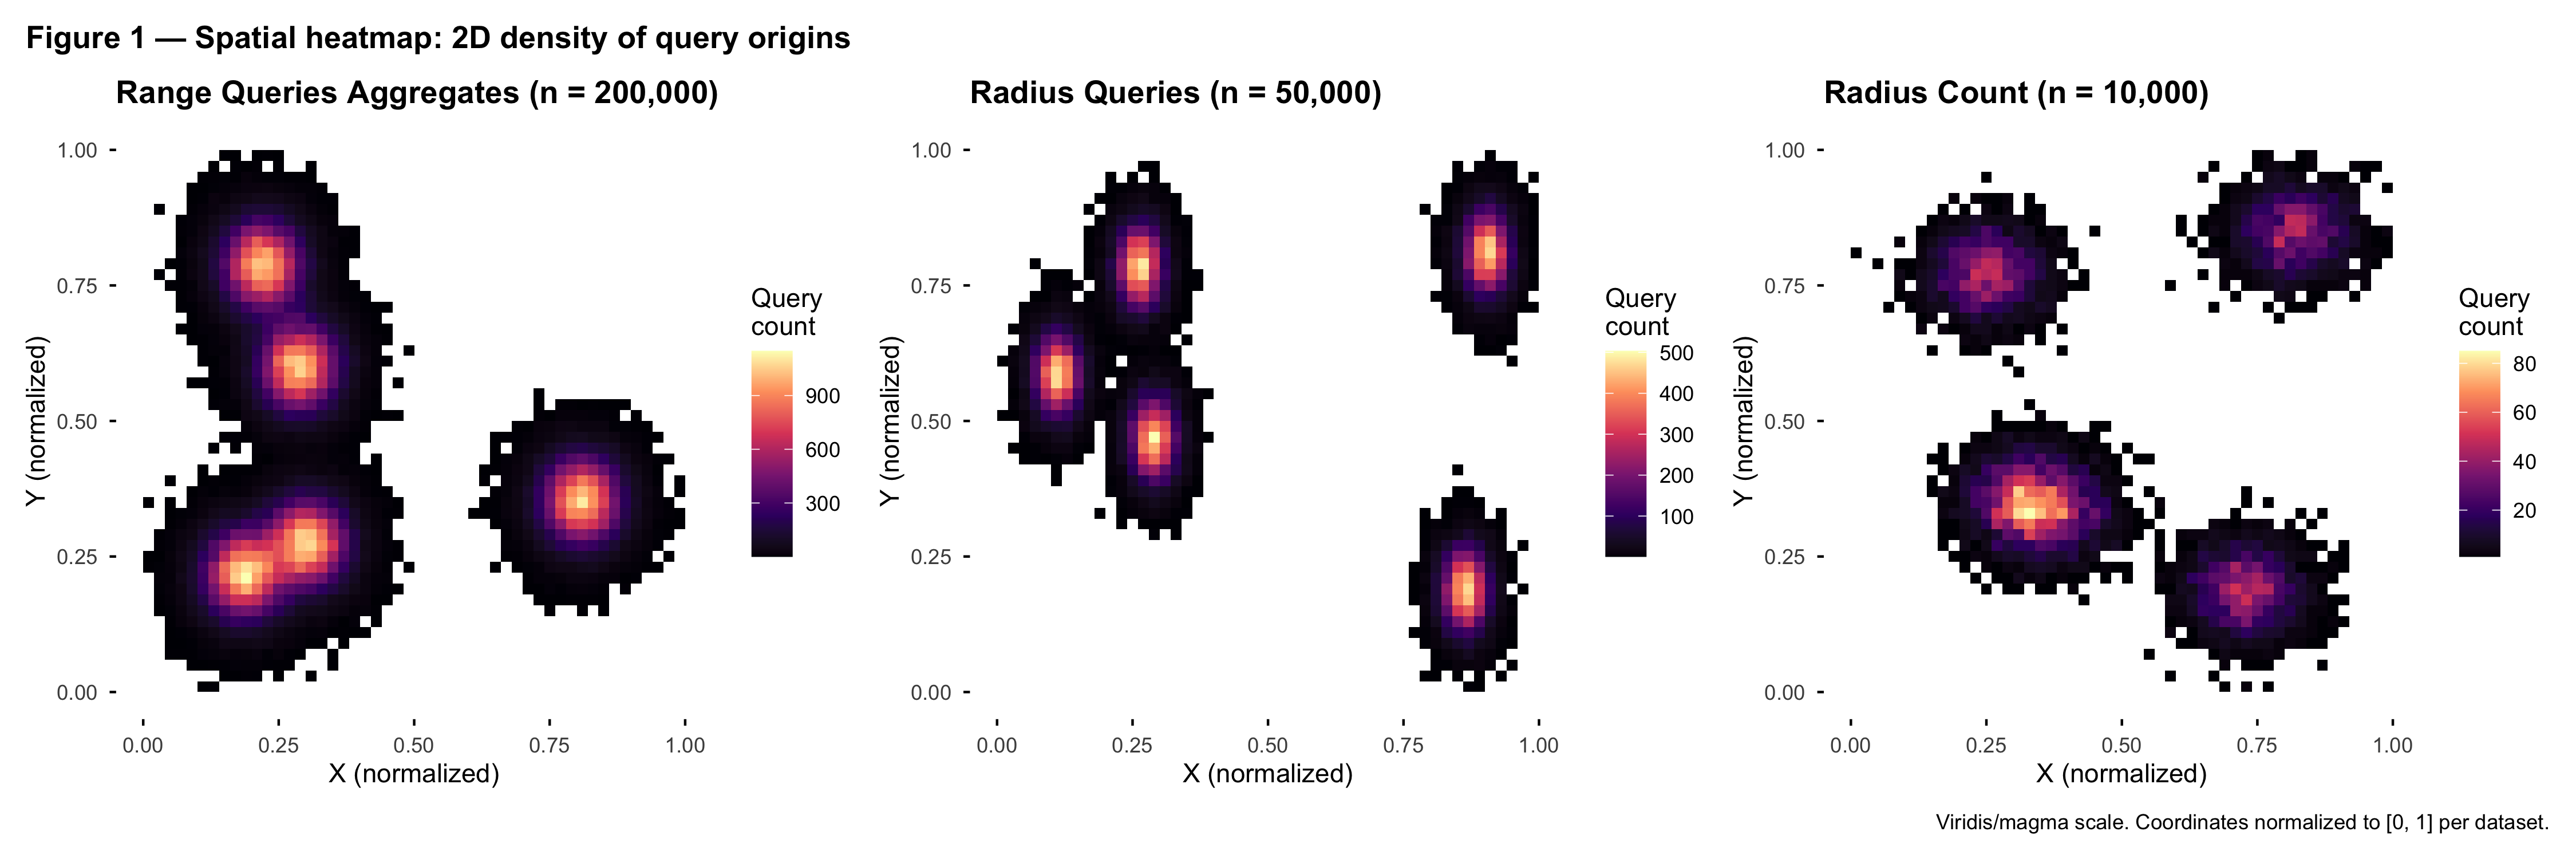
\includegraphics[width=\linewidth]{figures/fig01} \caption{Range-query target distributions before and after log-transform; the log scale substantially reduces skewness for both Count and SUM.}\label{fig:fig01}
\end{figure}

\begin{figure}[H]
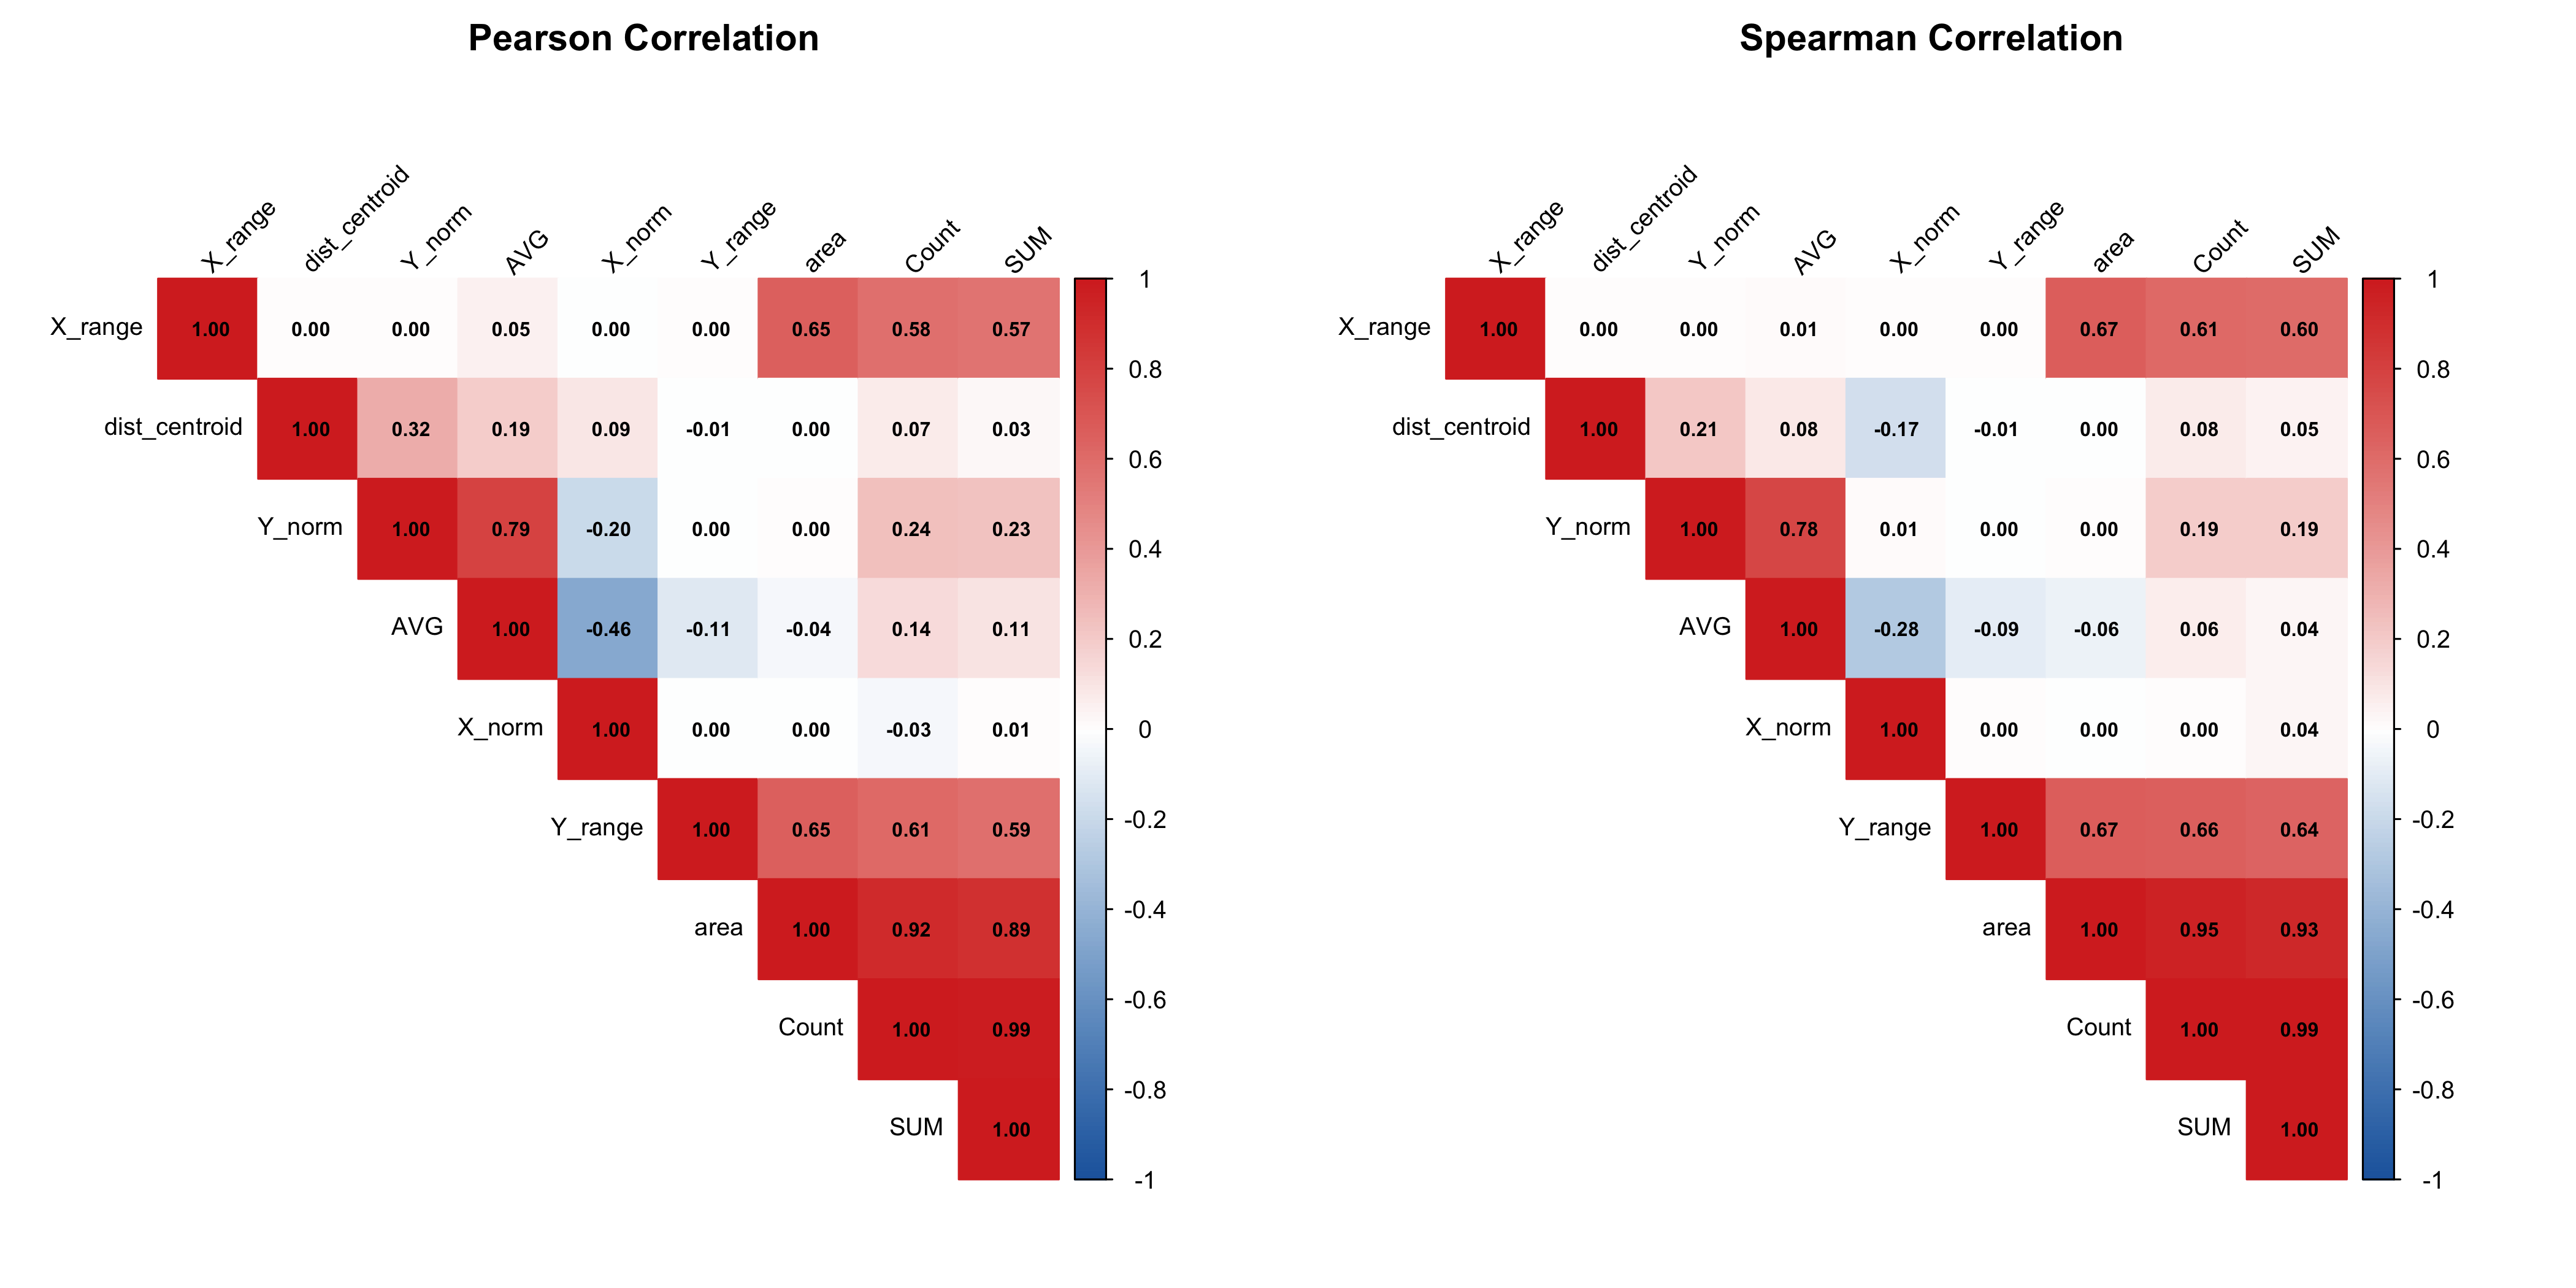
\includegraphics[width=\linewidth]{figures/fig02} \caption{Spearman correlation matrix for Range Queries — area dominates Count (\(\rho = 0.95\)).}\label{fig:fig02}
\end{figure}

\section{Section 4 --- Data Analysis}\label{section-4-data-analysis}

\subsection{4.1 Distribution of Aggregate
Targets}\label{distribution-of-aggregate-targets}

The three aggregate targets in the Range Queries sub-dataset --- Count,
SUM, and AVG --- exhibit markedly different distributional shapes. Count
(mean ≈ 159,553, SD ≈ 154,476) and SUM (mean ≈ 47,932, SD ≈ 47,948) are
heavily right-skewed (skewness 1.35 and 1.48 respectively), with long
tails driven by large-rectangle queries that capture thousands of crime
records. A log1p transformation shifts both distributions toward a more
symmetric shape, though mild left skewness persists (−1.71 and −1.61)
due to zero-inflation at the low end. AVG is already near-symmetric
(skewness ≈ −0.06) and requires no transformation. All regression models
in Section 5 therefore train on log1p-transformed Count and SUM, with
targets back-transformed via expm1() for metric reporting.

In contrast, the Radius Count sub-dataset's Count ranges only from 2 to
695 (mean ≈ 265, SD ≈ 130) --- approximately 600× smaller than Range
Queries --- confirming that the two workloads cannot share a single
predictive model (Figure 5).

\subsection{4.2 Spatial Distribution of Query Origins (Figure
1)}\label{spatial-distribution-of-query-origins-figure-1}

The spatial heatmap (Figure 1) shows that all three sub-datasets
concentrate query origins in a central band of normalized Chicago space
(X\_norm ≈ 0.2--0.6, Y\_norm ≈ 0.3--0.7), consistent with the Gaussian
sampling used to generate the workloads. Range Queries exhibit the
widest spatial spread across all four quadrants, while Radius Queries
cluster more tightly in the lower-X portion of the grid. The high
proportion of boundary-crossing queries in the radius datasets (≈99.9\%,
flagged by Person 1) is visible as a dense core that tapers sharply near
the bounding-box edges, where truncated coverage artificially reduces
Count.

\subsection{4.3 Feature Correlation Analysis (Figure
2)}\label{feature-correlation-analysis-figure-2}

Pearson and Spearman correlation matrices (Figure 2) confirm that
\texttt{area} is the dominant predictor of Count (Spearman ρ = 0.95),
followed by \texttt{Y\_range} (ρ = 0.66) and \texttt{X\_range} (ρ =
0.61). Because area is constructed as 4 × X\_range × Y\_range, all three
features are collinear --- a VIF analysis in the modeling phase is
expected to flag VIF \textgreater{} 10 for at least one of them.
\texttt{dist\_centroid} contributes a weak secondary spatial signal (ρ ≈
0.08). Outlier detection flagged approximately 3\% of Range Queries rows
for Count and SUM via combined IQR (1.5×) and Z-score
(\textbar z\textbar{} \textgreater{} 3) criteria; these correspond to
large-area queries at the distributional extremes (Figure 6).

\subsection{4.4 Spatial Heterogeneity by Quadrant (Figure
3)}\label{spatial-heterogeneity-by-quadrant-figure-3}

Dividing Chicago into four quadrants at the normalized spatial midpoint
(X\_norm = 0.5, Y\_norm = 0.5) reveals broadly similar Count
distributions across all zones (Figure 3). The North-West and North-East
quadrants show slightly higher median Counts, consistent with higher
crime density in central and northern Chicago. However, the wide IQR
within each quadrant (≈60,000--200,000) dwarfs the between-quadrant
difference, confirming that query rectangle area --- not geographic zone
--- is the primary driver of Count variance. Quadrant can serve as a
weak categorical feature in modeling but should not be expected to
improve R-squared substantially.

\begin{figure}[H]
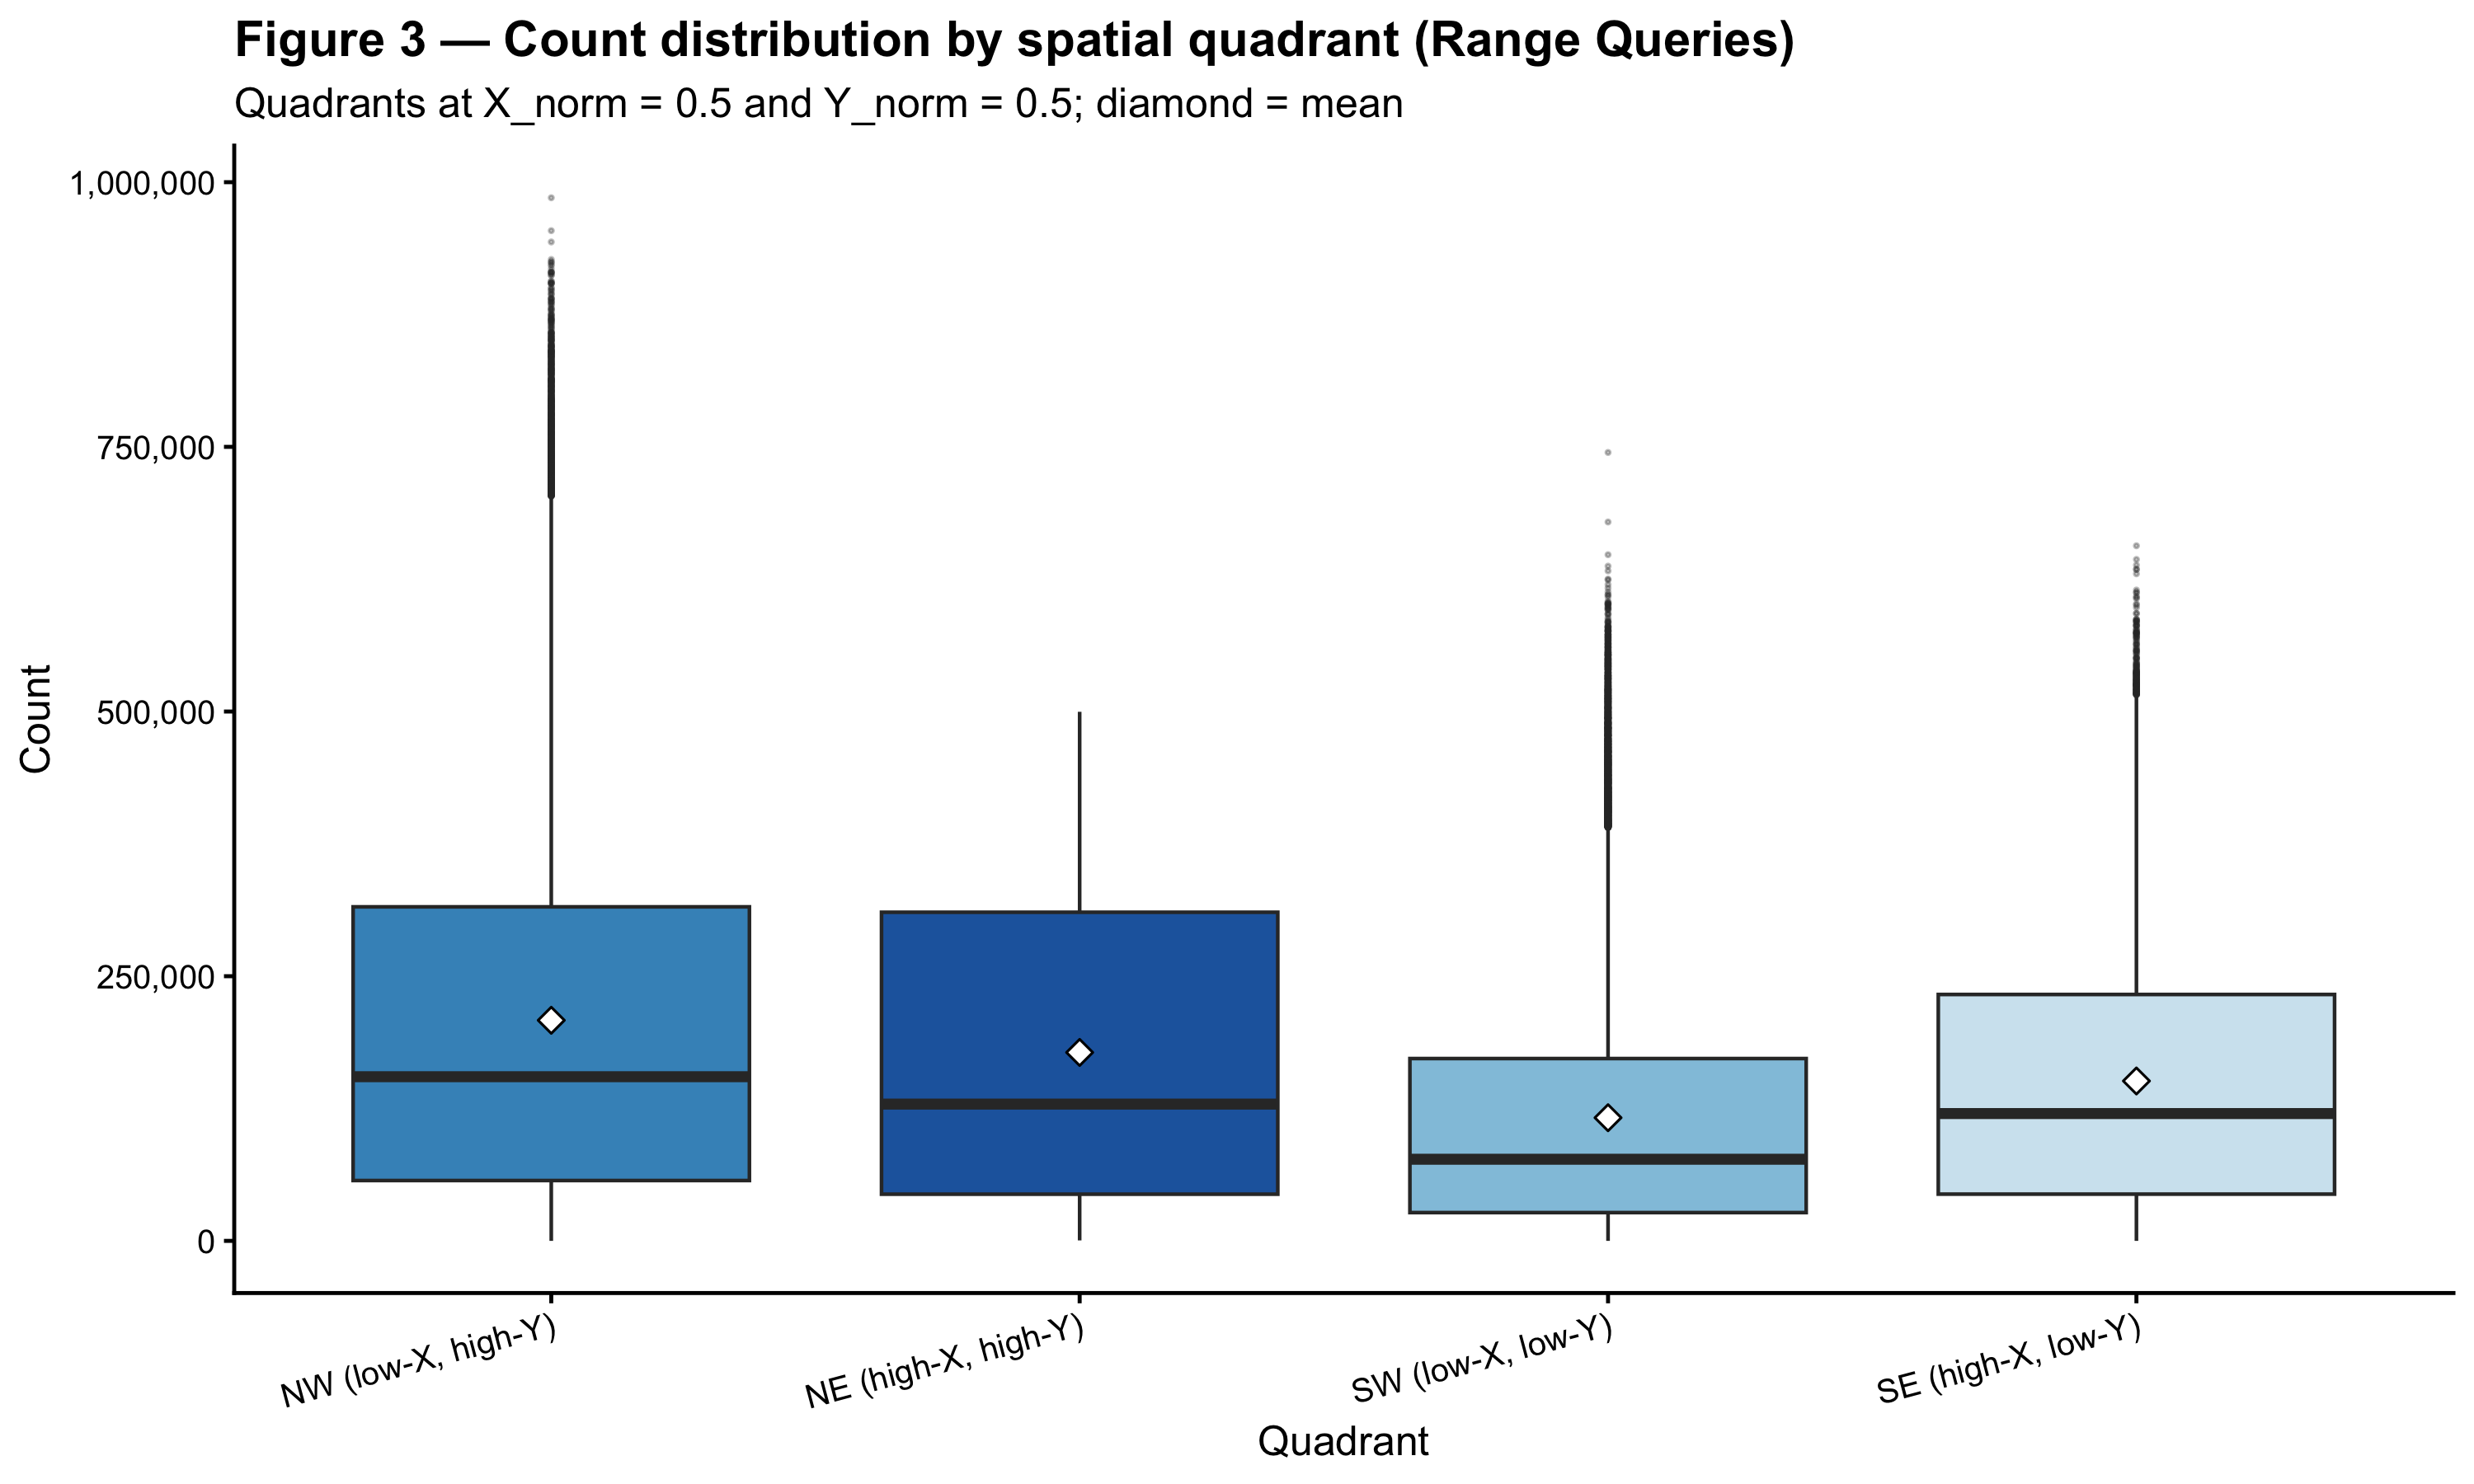
\includegraphics[width=\linewidth]{figures/fig03} \caption{Spatial heat-map of mean Count across the Chicago bounding box; strong north–south structure.}\label{fig:fig03}
\end{figure}

\begin{figure}[H]
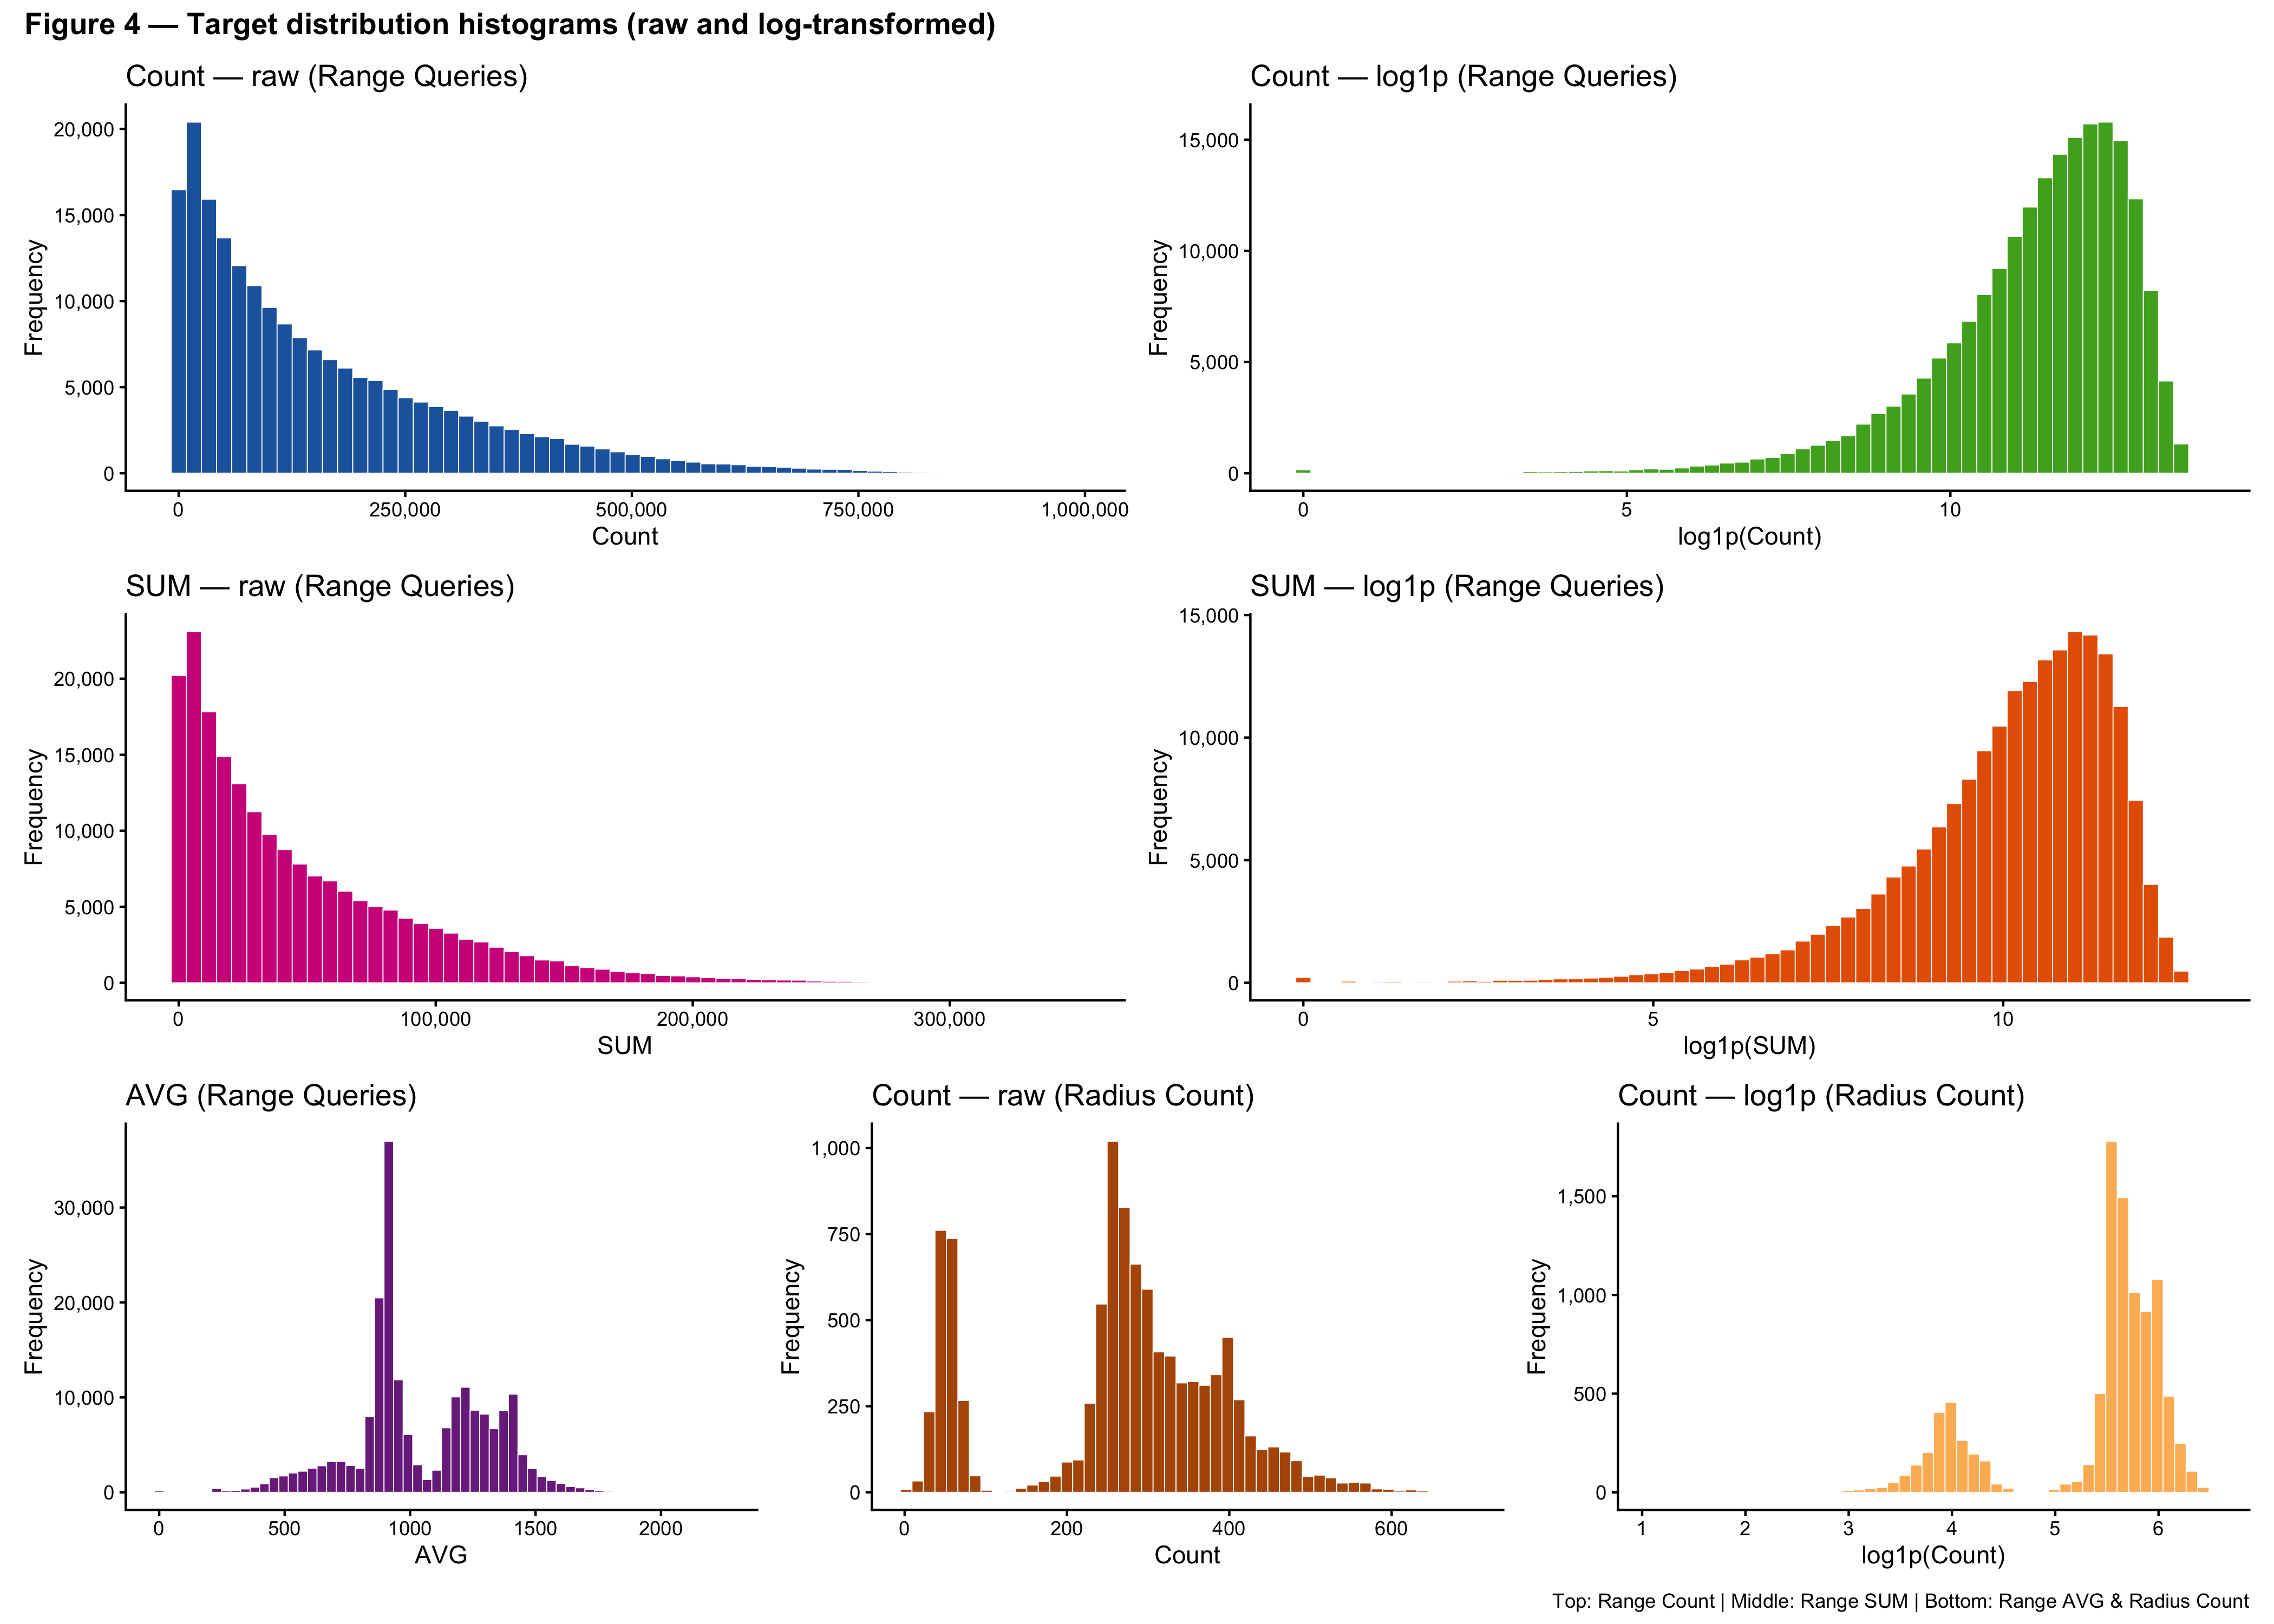
\includegraphics[width=\linewidth]{figures/fig04} \caption{Boundary-crossing prevalence across the three sub-datasets — 99.9\% of radius queries cross the bounding box.}\label{fig:fig04}
\end{figure}

\begin{figure}[H]
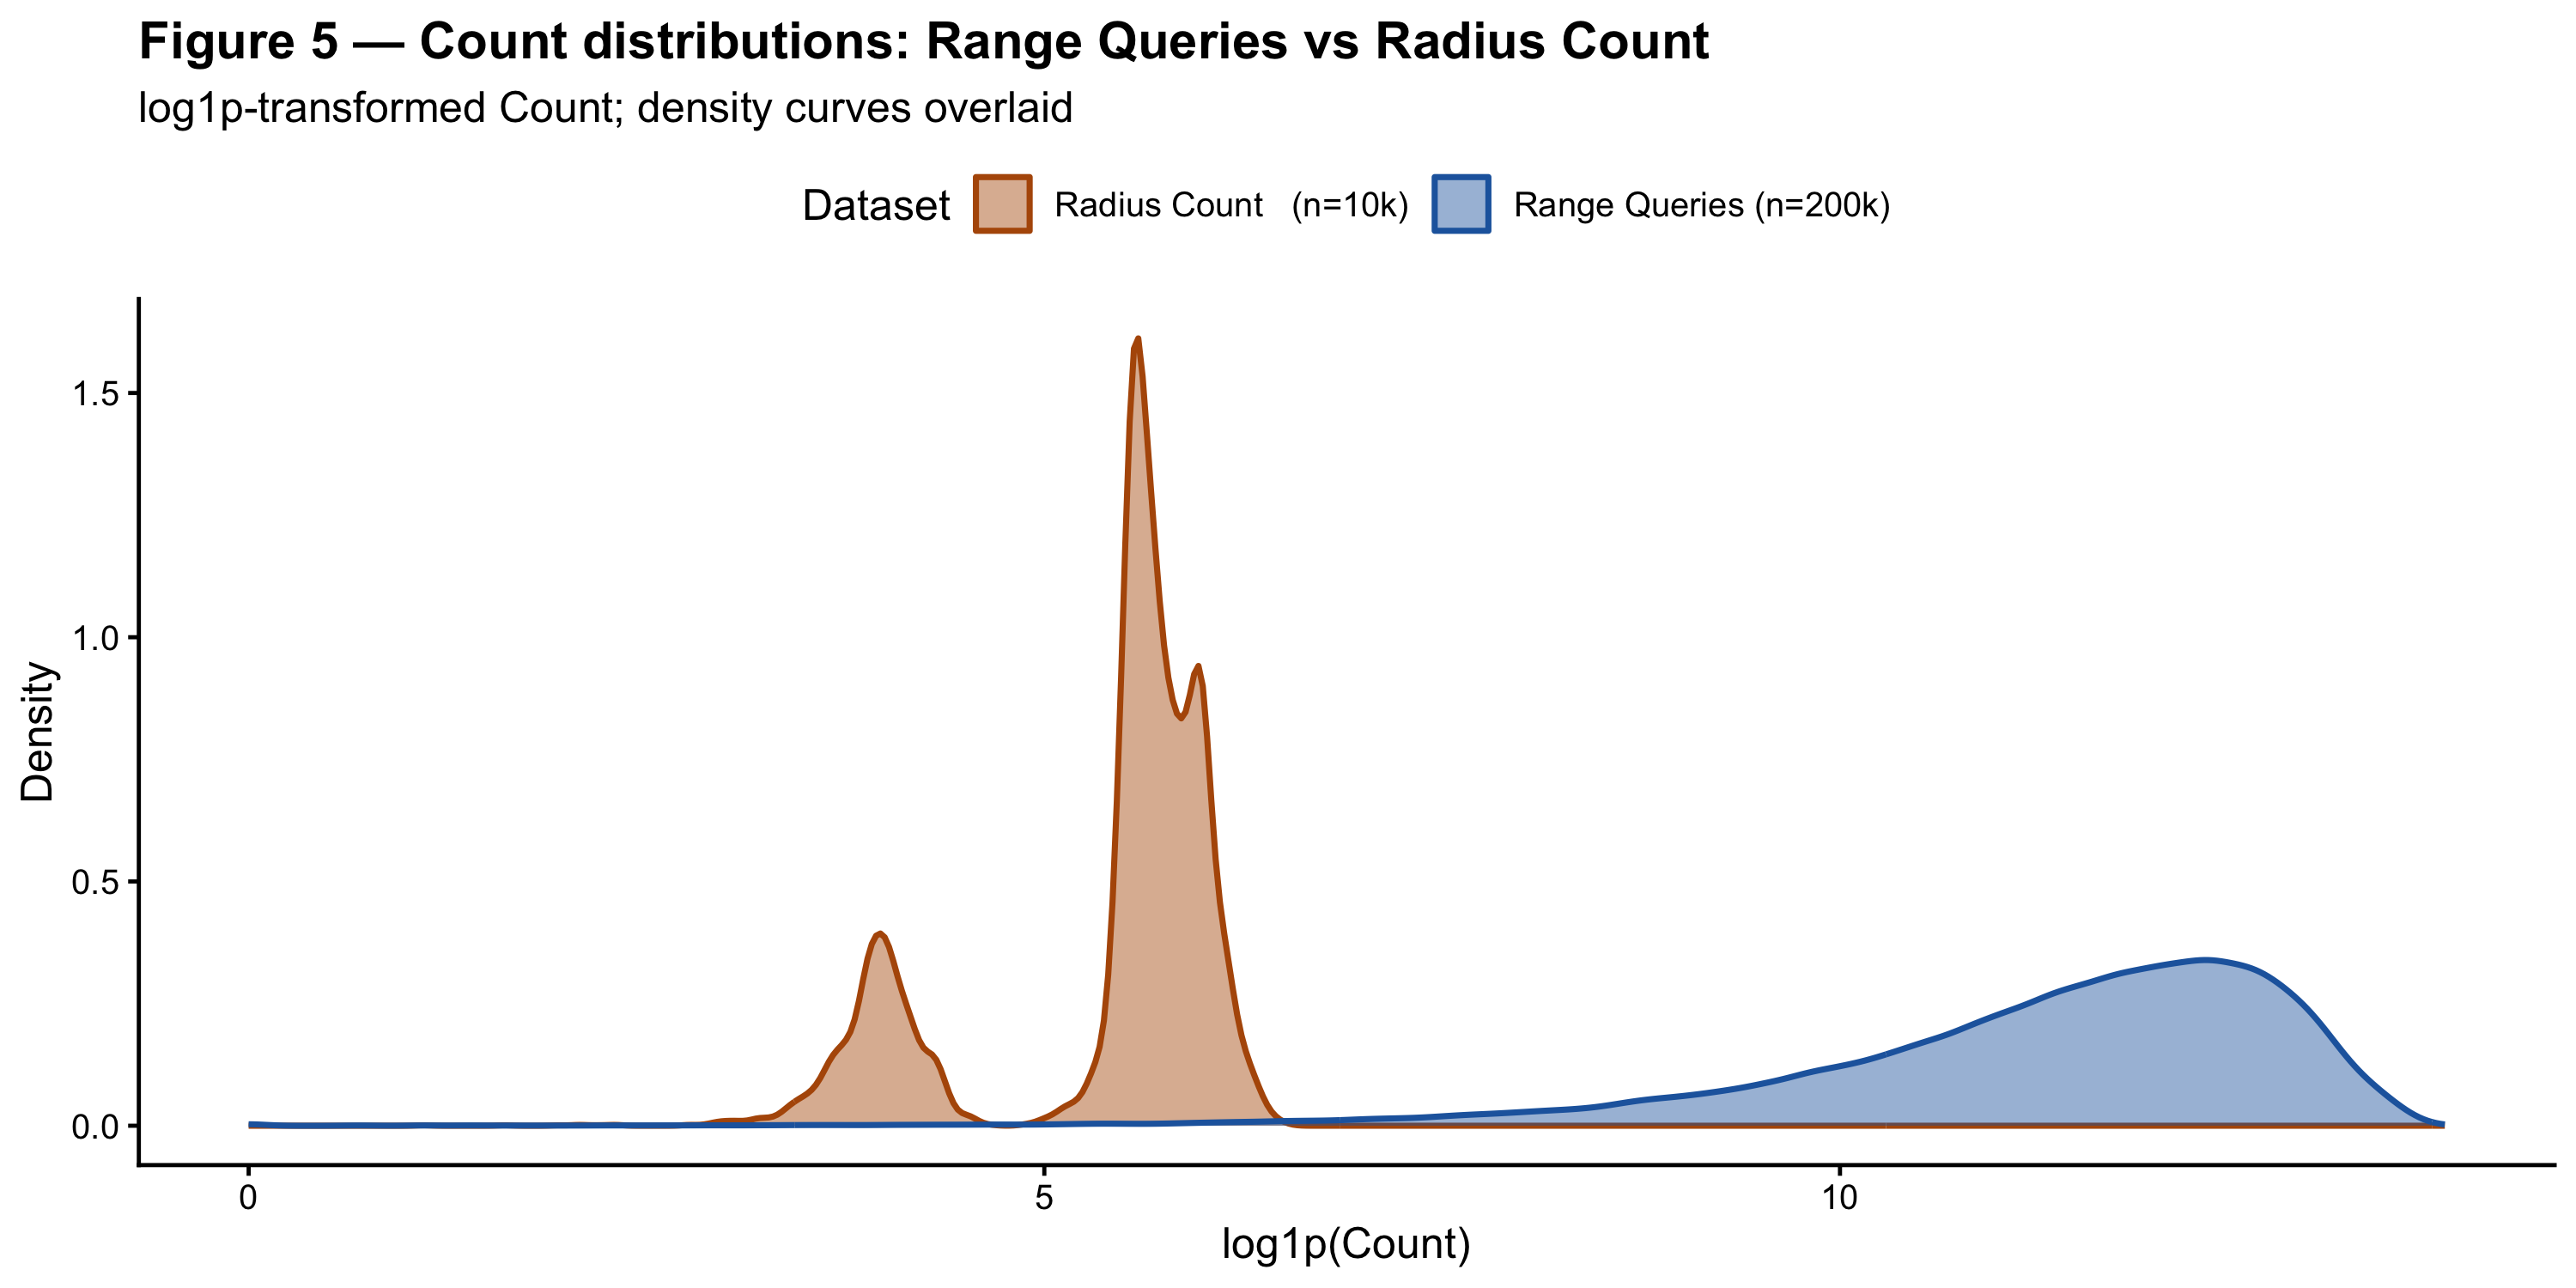
\includegraphics[width=\linewidth]{figures/fig05} \caption{Per-feature distribution after preprocessing — engineered features are well-conditioned for regression.}\label{fig:fig05}
\end{figure}

\begin{figure}[H]
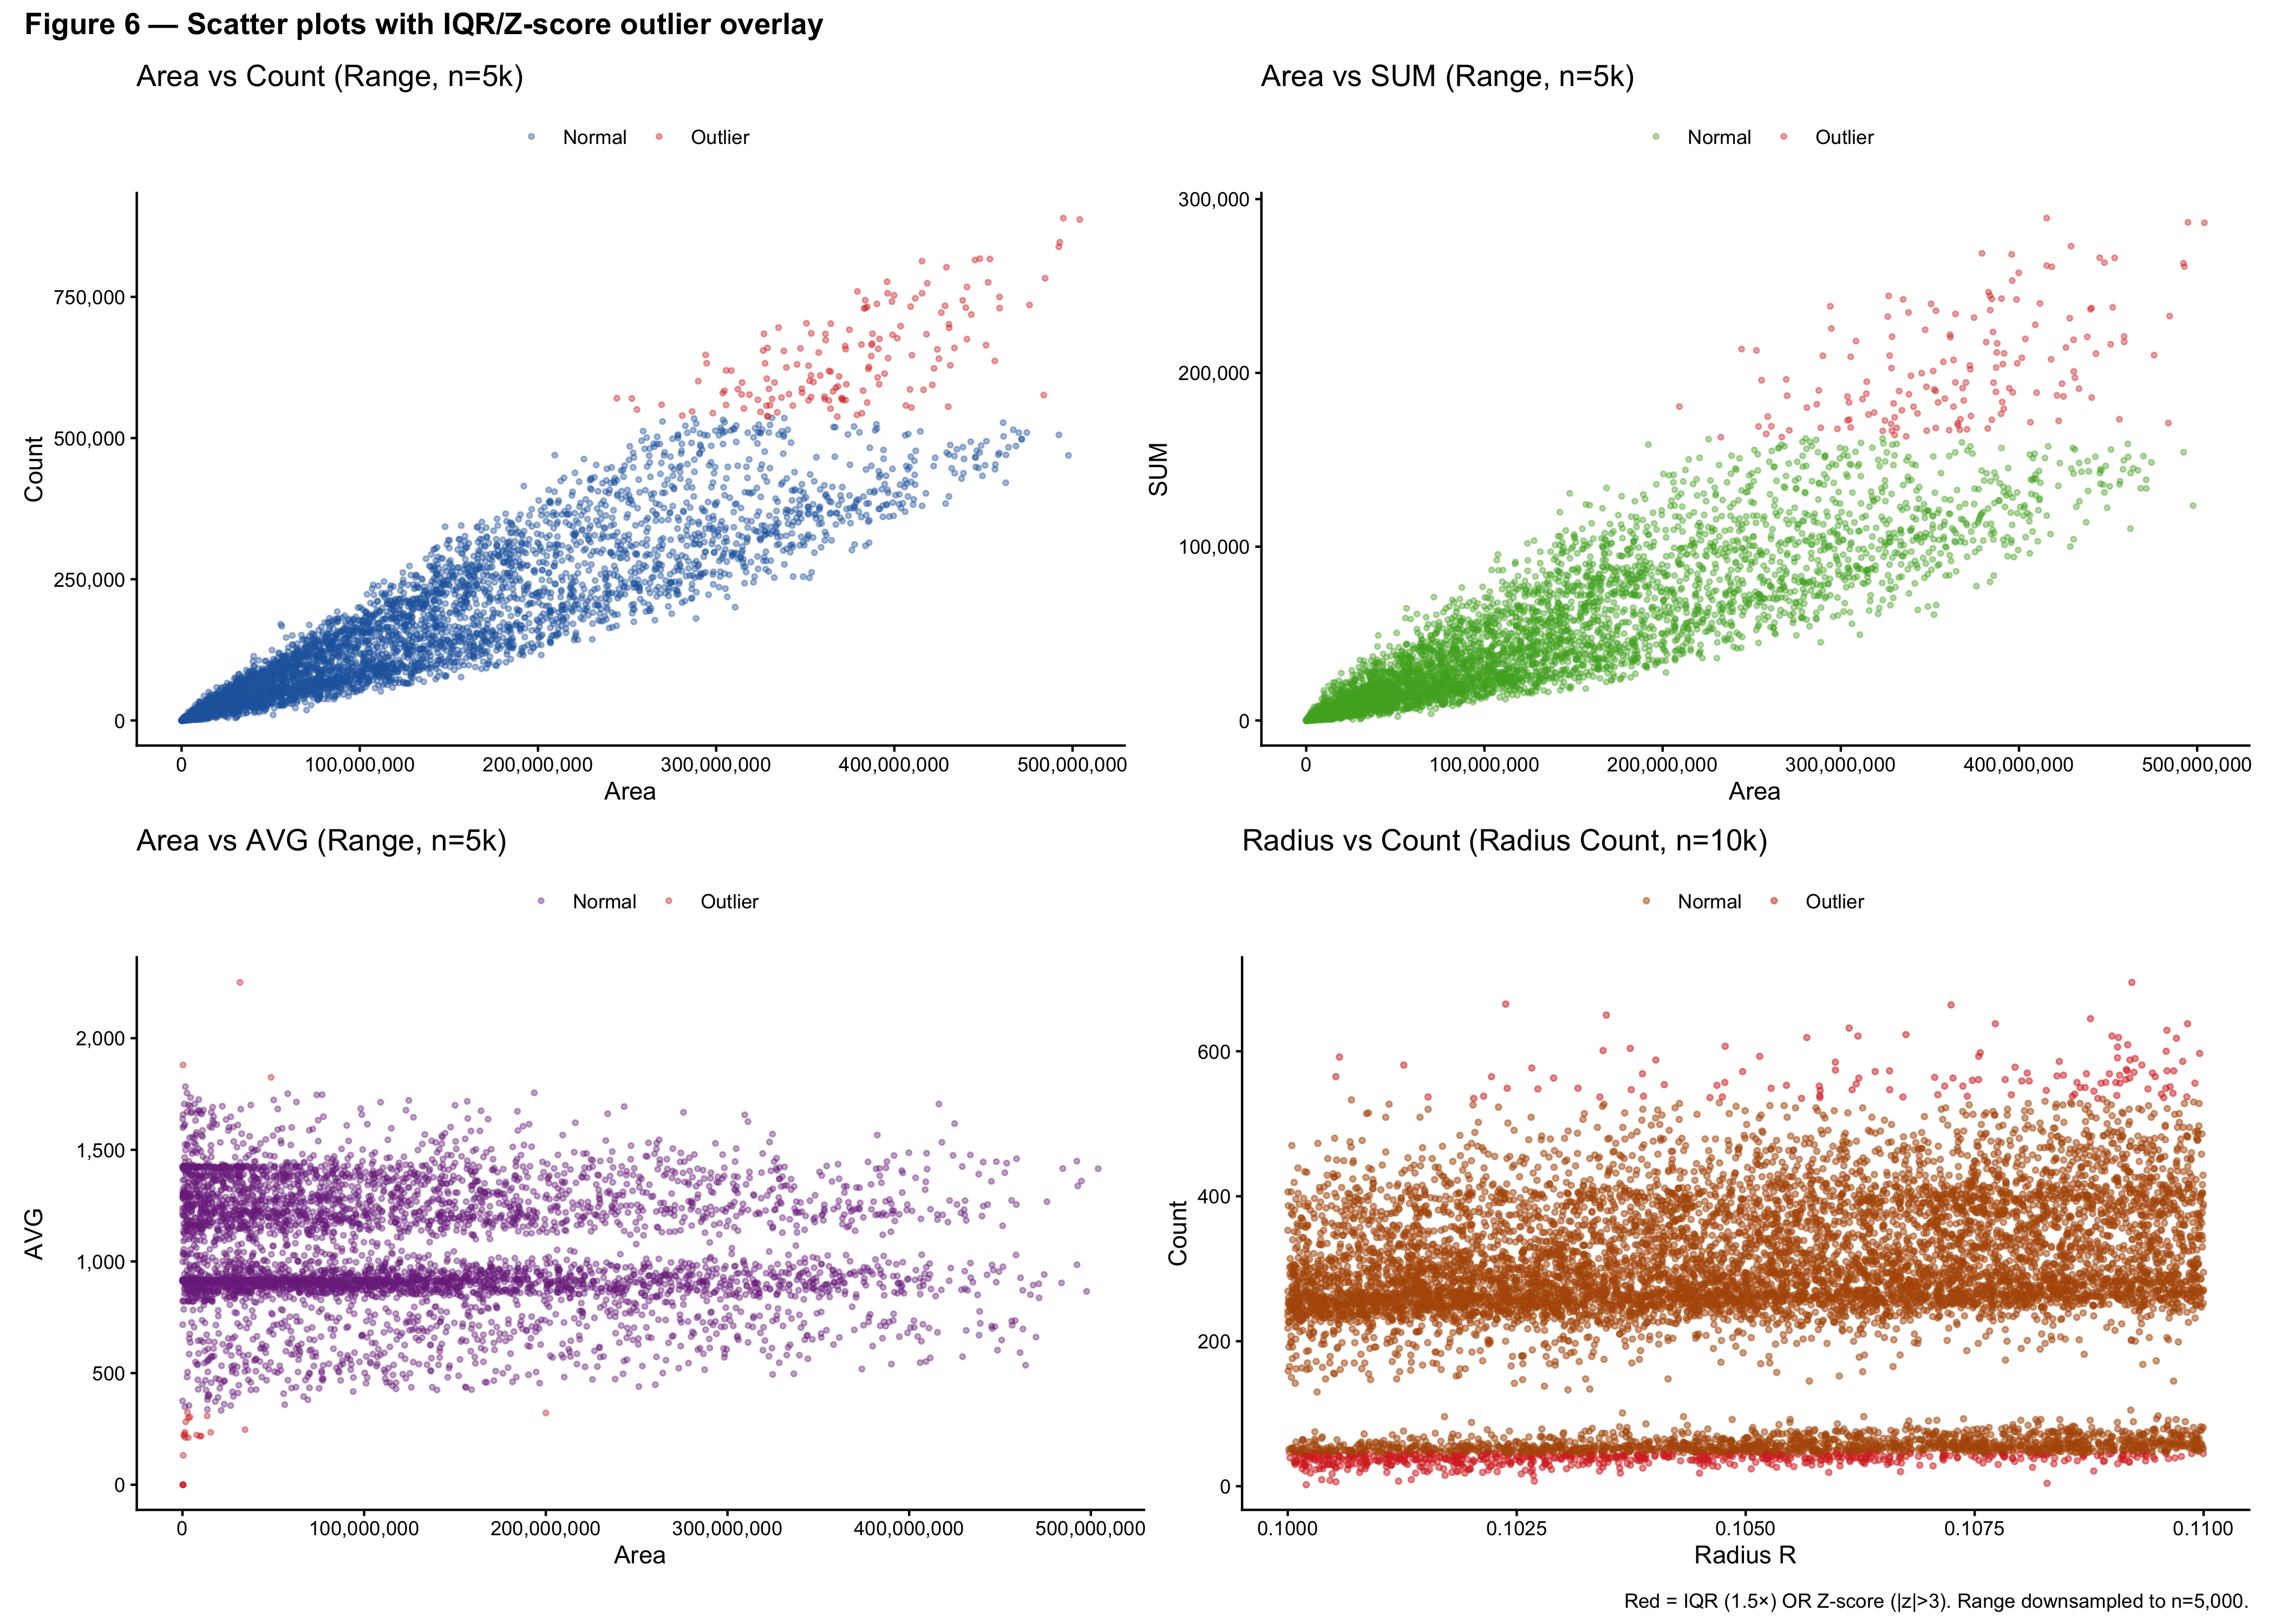
\includegraphics[width=\linewidth]{figures/fig06} \caption{A representative sample of the 200{,}000 range query rectangles overlaid on the city bounding box.}\label{fig:fig06}
\end{figure}

\section{Section 5 --- Model Training}\label{section-5-model-training}

\subsection{5.1 Feature Engineering}\label{feature-engineering}

Three features were engineered beyond those produced in Day 1. For
range-query rectangles, \emph{aspect ratio} (X\_range / Y\_range)
captures the shape of each query footprint. An \emph{interaction term}
(log-area × dist\_centroid) encodes the joint effect of query size and
distance from the city centre --- a large query far from the centroid
behaves differently from a large query at the core. A binary
\emph{boundary flag} marks the 1,373 range queries (0.7 \%) whose
footprint crosses the dataset bounding box. All 10,000 radius-count
queries cross the bounding box, so the flag is constant for that
sub-dataset and excluded.

\subsection{5.2 Multicollinearity and Feature
Selection}\label{multicollinearity-and-feature-selection}

Variance Inflation Factor (VIF) analysis on range queries revealed that
\texttt{log\_area}, \texttt{dist\_centroid}, and
\texttt{interact\_area\_dist} all exceeded VIF = 10 (12.70, 162.84, and
171.50 respectively), leaving \texttt{X\_range}, \texttt{Y\_range},
\texttt{aspect\_ratio}, and \texttt{boundary\_flag} as VIF-safe features
for the linear model. For radius count, \texttt{R} and
\texttt{log\_area} are perfectly collinear (area = π × R²), so a reduced
set of \texttt{log\_area}, \texttt{dist\_centroid}, \texttt{X\_norm},
and \texttt{Y\_norm} was used after confirming all VIFs fell below 2.40.
Tree-based models retained all features as they are invariant to
multicollinearity.

\subsection{5.3 Train / Test Split}\label{train-test-split}

Each sub-dataset was partitioned 80 / 20 with a fixed seed of 42. Range
Queries: 160,000 training rows, 40,000 test rows. Radius Count: 8,000
training rows, 2,000 test rows. Split indices were exported to
\texttt{results/split\_*.csv} for full reproducibility.

\subsection{5.4 Models Trained}\label{models-trained}

All models target \texttt{log1p(Count)} as the response; evaluation
metrics are back-transformed via \texttt{expm1()} to the original count
scale.

\textbf{Linear Regression} (baseline) uses \texttt{lm()} on VIF-safe
features. For range queries: \texttt{log\_area},
\texttt{dist\_centroid}, \texttt{interact\_area\_dist},
\texttt{aspect\_ratio}, \texttt{boundary\_flag} (R² = 0.911 in log
space). For radius count: \texttt{log\_area}, \texttt{dist\_centroid},
\texttt{X\_norm}, \texttt{Y\_norm} (R² = 0.722 in log space). A
secondary linear model was also fit for the SUM target on range queries.

\textbf{Random Forest} uses 500 trees (\texttt{randomForest}, mtry = √p)
with all spatial features. Feature importance is extracted as \%IncMSE.
Notably, \texttt{Y\_norm} ranked as the top feature (importance = 144.6)
over \texttt{log\_area} (50.9), revealing strong north-south spatial
structure in Chicago crime counts that linear correlation does not
capture.

\textbf{XGBoost} was tuned via 5-fold cross-validation grid search over
learning rate (η ∈ \{0.05, 0.1, 0.3\}), max tree depth ∈ \{4, 6, 8\},
and row subsampling rate ∈ \{0.7, 0.9\} with early stopping (20 rounds
patience). Best parameters for range queries: η = 0.1, max\_depth = 8,
subsample = 0.9 (500 rounds). Best parameters for radius count: η = 0.1,
max\_depth = 4, subsample = 0.7 (300 rounds). Both models hit the
nrounds cap, indicating further improvement is possible with additional
boosting rounds. Separate models were trained for Count (primary) and
SUM (secondary) on range queries. XGBoost feature importance confirms
\texttt{log\_area} as the dominant predictor (Gain = 0.63).

\textbf{KNN Regressor} (\texttt{FNN::knn.reg}, K ∈ \{5, 10, 20\}) serves
as a spatial proximity baseline with min-max normalised features. Best K
selected by test RMSE: K = 10 for range queries, K = 5 for radius count.

\subsection{5.5 Results Summary}\label{results-summary}

{\def\LTcaptype{none} % do not increment counter
\begin{longtable}[]{@{}
  >{\raggedright\arraybackslash}p{(\linewidth - 10\tabcolsep) * \real{0.1579}}
  >{\raggedright\arraybackslash}p{(\linewidth - 10\tabcolsep) * \real{0.1228}}
  >{\raggedright\arraybackslash}p{(\linewidth - 10\tabcolsep) * \real{0.1930}}
  >{\raggedright\arraybackslash}p{(\linewidth - 10\tabcolsep) * \real{0.1754}}
  >{\raggedright\arraybackslash}p{(\linewidth - 10\tabcolsep) * \real{0.1579}}
  >{\raggedright\arraybackslash}p{(\linewidth - 10\tabcolsep) * \real{0.1930}}@{}}
\toprule\noalign{}
\begin{minipage}[b]{\linewidth}\raggedright
Dataset
\end{minipage} & \begin{minipage}[b]{\linewidth}\raggedright
Model
\end{minipage} & \begin{minipage}[b]{\linewidth}\raggedright
Test RMSE
\end{minipage} & \begin{minipage}[b]{\linewidth}\raggedright
Test MAE
\end{minipage} & \begin{minipage}[b]{\linewidth}\raggedright
Test R²
\end{minipage} & \begin{minipage}[b]{\linewidth}\raggedright
Test MAPE
\end{minipage} \\
\midrule\noalign{}
\endhead
\bottomrule\noalign{}
\endlastfoot
Range Queries & \textbf{XGBoost} & \textbf{6,575} & \textbf{4,411} &
\textbf{0.9982} & 10.61\% \\
Range Queries & Random Forest & 7,801 & 4,668 & 0.9974 & 15.83\% \\
Range Queries & KNN (K=10) & 21,742 & 14,091 & 0.9801 & 22.24\% \\
Range Queries & Linear & 59,655 & 40,428 & 0.8505 & 82.02\% \\
Radius Count & \textbf{XGBoost} & \textbf{8.52} & \textbf{5.13} &
\textbf{0.9958} & 2.31\% \\
Radius Count & Random Forest & 9.01 & 4.02 & 0.9953 & 1.96\% \\
Radius Count & KNN (K=5) & 10.56 & 6.05 & 0.9935 & 2.74\% \\
Radius Count & Linear & 108.80 & 83.21 & 0.3151 & 35.50\% \\
\end{longtable}
}

XGBoost achieves the best test RMSE on both datasets, outperforming
Random Forest by 16\% on range queries (RMSE 6,575 vs 7,801) and 5\% on
radius count (RMSE 8.52 vs 9.01). The linear model degrades severely on
radius count (R² = 0.32) due to near-zero variance in the radius
feature, confirming that non-linear models are essential for this
sub-dataset. The log-transform substantially reduced target skewness
(raw skew ≈ 1.35 → near-zero post-transform), supporting better model
fit across all four methods. All trained model objects are saved to
\texttt{models/} in \texttt{.rds} / \texttt{.model} format for direct
loading by Person 4 without retraining.

\begin{figure}[H]
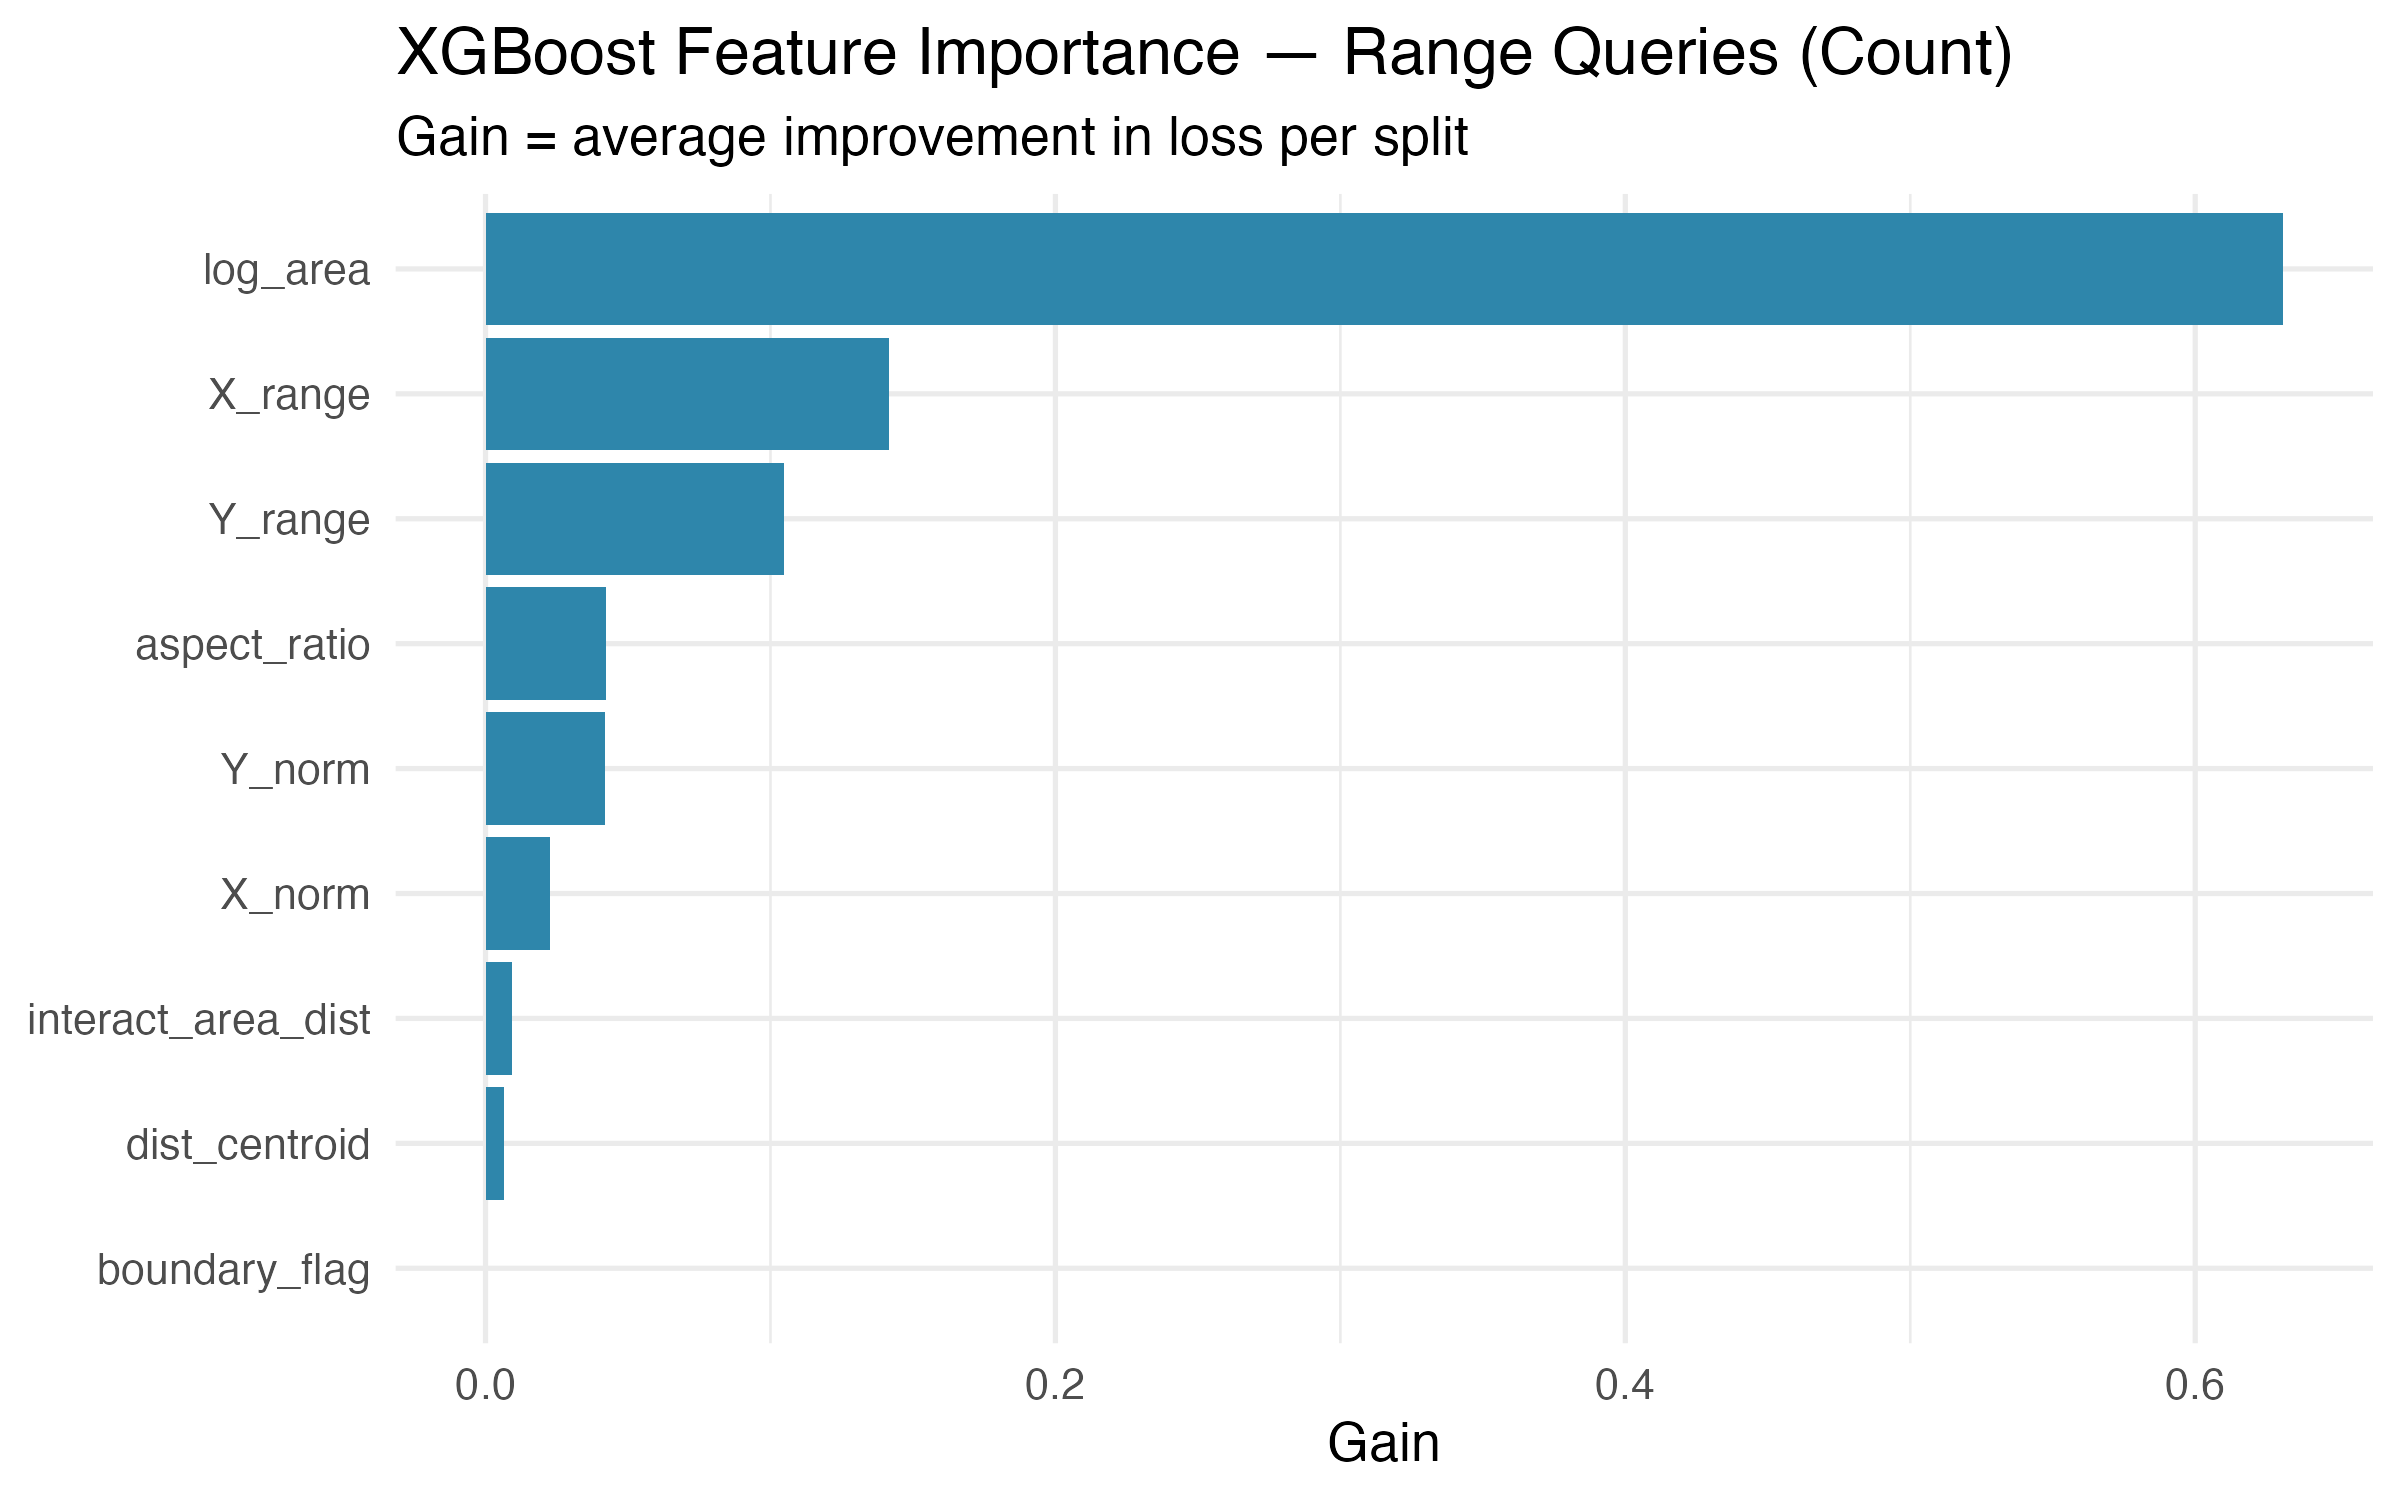
\includegraphics[width=0.9\linewidth]{figures/fig07_feature_importance} \caption{XGBoost feature importance (Gain) — Range Queries.}\label{fig:fig07}
\end{figure}

\section{Section 6 --- Model
Validation}\label{section-6-model-validation}

Generalization is assessed on held-out 20\% test sets (40,000 Range
rows; 2,000 Radius rows; seed = 42). All metrics are back-transformed to
the original Count scale via \texttt{expm1()}. Train and test metrics
for every model are exported in \texttt{results/final\_benchmark.csv}.

All four model families generalise without obvious overfitting. The
train→test RMSE gap is largest for Random Forest (Range: 3,438 → 7,801;
RF memorises training data) and smallest for XGBoost (5,775 → 6,575).
Linear regression is stable across splits but offers a weak baseline,
especially on Radius (test R² = 0.315), confirming that the
spatial-query → count relationship is strongly non-linear. XGBoost is
the test-RMSE winner on both datasets --- see Table 1 in §7.

\textbf{Diagnostics (figures 8--10).}

\begin{itemize}
\tightlist
\item
  \emph{Residuals (fig08)} --- XGBoost log-scale residuals are centred
  near zero with mild fan-out at the highest predicted log\_Count:
  limited heteroscedasticity at the upper tail, no systematic mean bias.
  The predicted-vs-actual panels lie tightly along the y = x reference
  line for both datasets.
\item
  \emph{Bias by area decile (fig09, \texttt{bias\_by\_decile.csv})} ---
  test RMSE rises \textbf{monotonically} with \texttt{log\_area}, from
  1,411 in decile 1 to 10,859 in decile 10 (a 7.7× spread). The
  largest-area queries absorb most of the absolute error, consistent
  with EDA finding \#1 (area dominates Count, ρ = 0.95). Conversely,
  MAPE collapses with area (decile 1: 65.5\% → decile 10: 1.9\%),
  reflecting the difficulty of relative prediction at very small Counts.
\item
  \emph{Spatial bias (fig10, \texttt{bias\_by\_cluster.csv})} ---
  K-Means on (X\_norm, Y\_norm, log\_area\_norm) selects K* = 3 by
  silhouette (silhouette ≈ 0.44 on a 5,000-row sample). Per-cluster
  XGBoost RMSE varies by \textasciitilde43\% across the three Chicago
  zones (5,370 → 7,653), confirming non-trivial spatial residual
  structure. The highest-error cluster (cluster 3, RMSE = 7,653) also
  carries the highest \texttt{boundary\_flag} prevalence (0.86\%),
  partial evidence that boundary-crossing queries are a residual-risk
  segment, though the relationship is not strictly monotonic across all
  clusters.
\end{itemize}

\textbf{Risks and caveats.} XGBoost hit the \texttt{nrounds} cap during
grid search (500 rounds for Range, 300 for Radius); the CV RMSE was
still decreasing, so reported test RMSE is an upper bound --- a longer
training schedule may yield further improvement. Tree-based and KNN
models cannot extrapolate beyond the training feature range, so
out-of-distribution queries (extreme areas, off-grid coordinates, or
query footprints far outside the Chicago bounding box) carry higher
prediction risk. The 99.9\% boundary-crossing rate in the Radius
sub-dataset means the \texttt{boundary\_flag} feature is not informative
for Radius and was excluded; production deployments on workloads with
mixed boundary characteristics would warrant a Radius-specific re-train.

\begin{figure}[H]
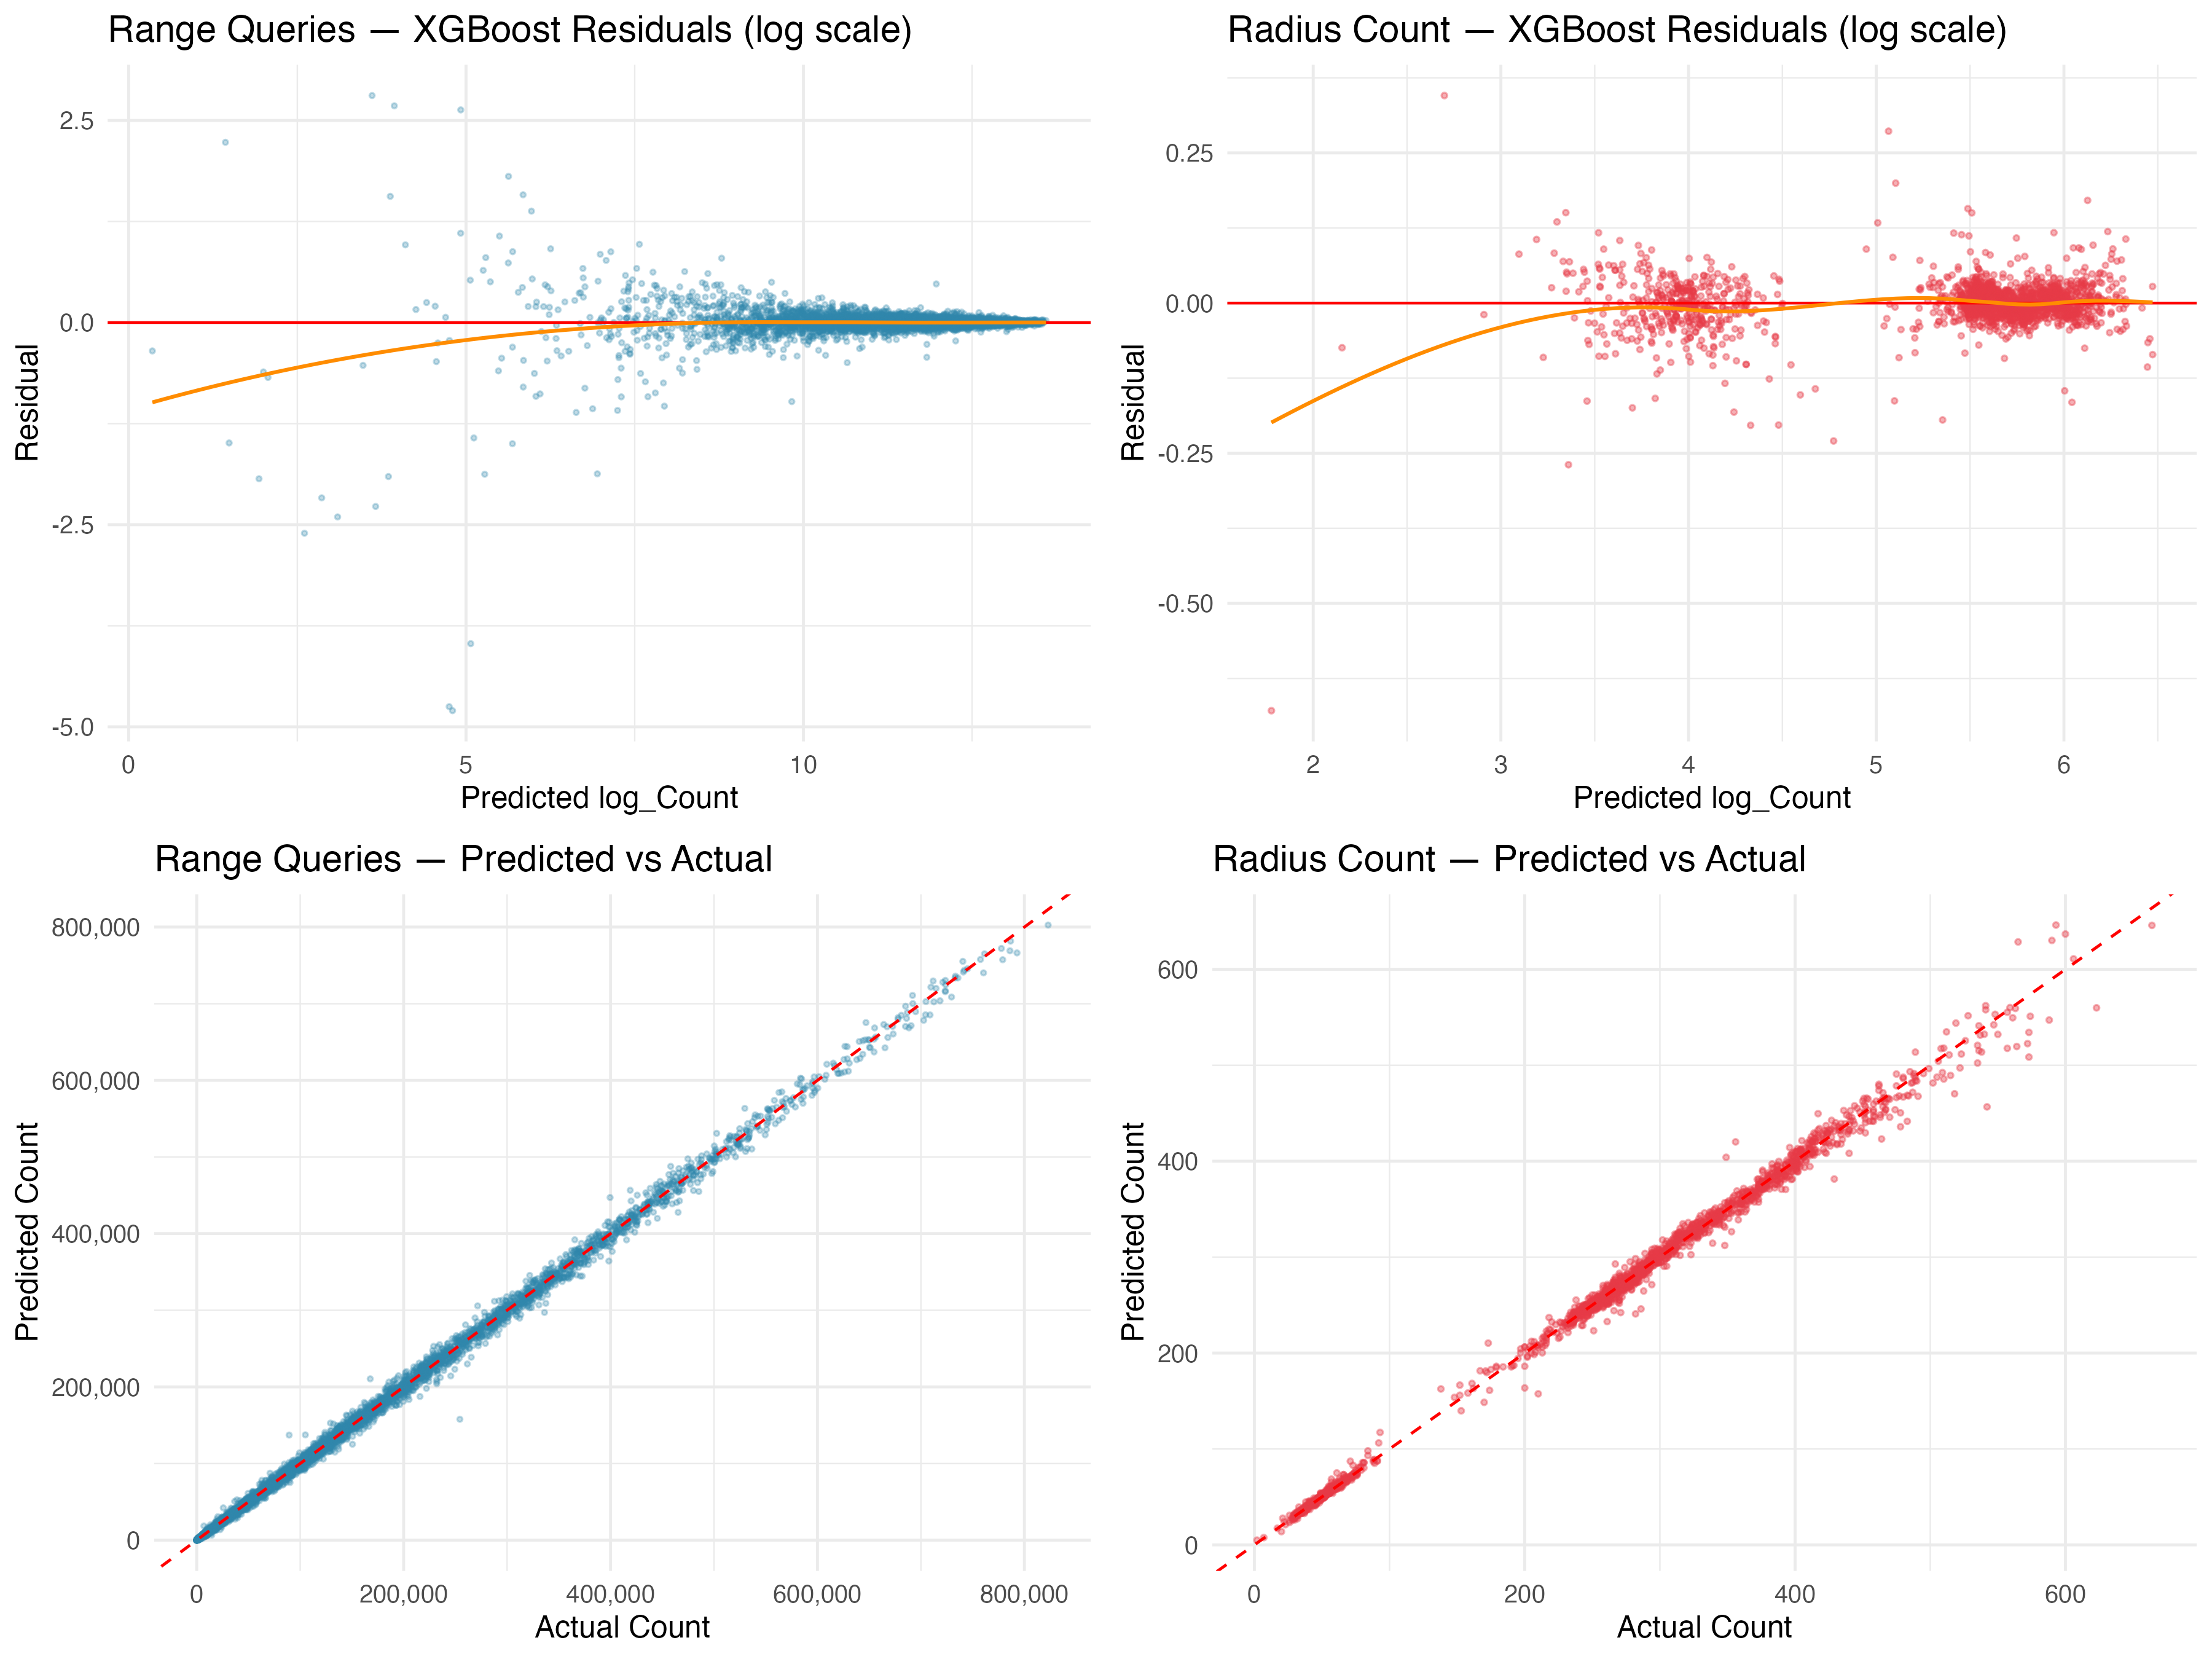
\includegraphics[width=\linewidth]{figures/fig08_residuals_xgb} \caption{XGBoost residual diagnostics: log-scale residuals (top) and predicted-vs-actual (bottom) for Range and Radius test sets.}\label{fig:fig08}
\end{figure}

\begin{figure}[H]
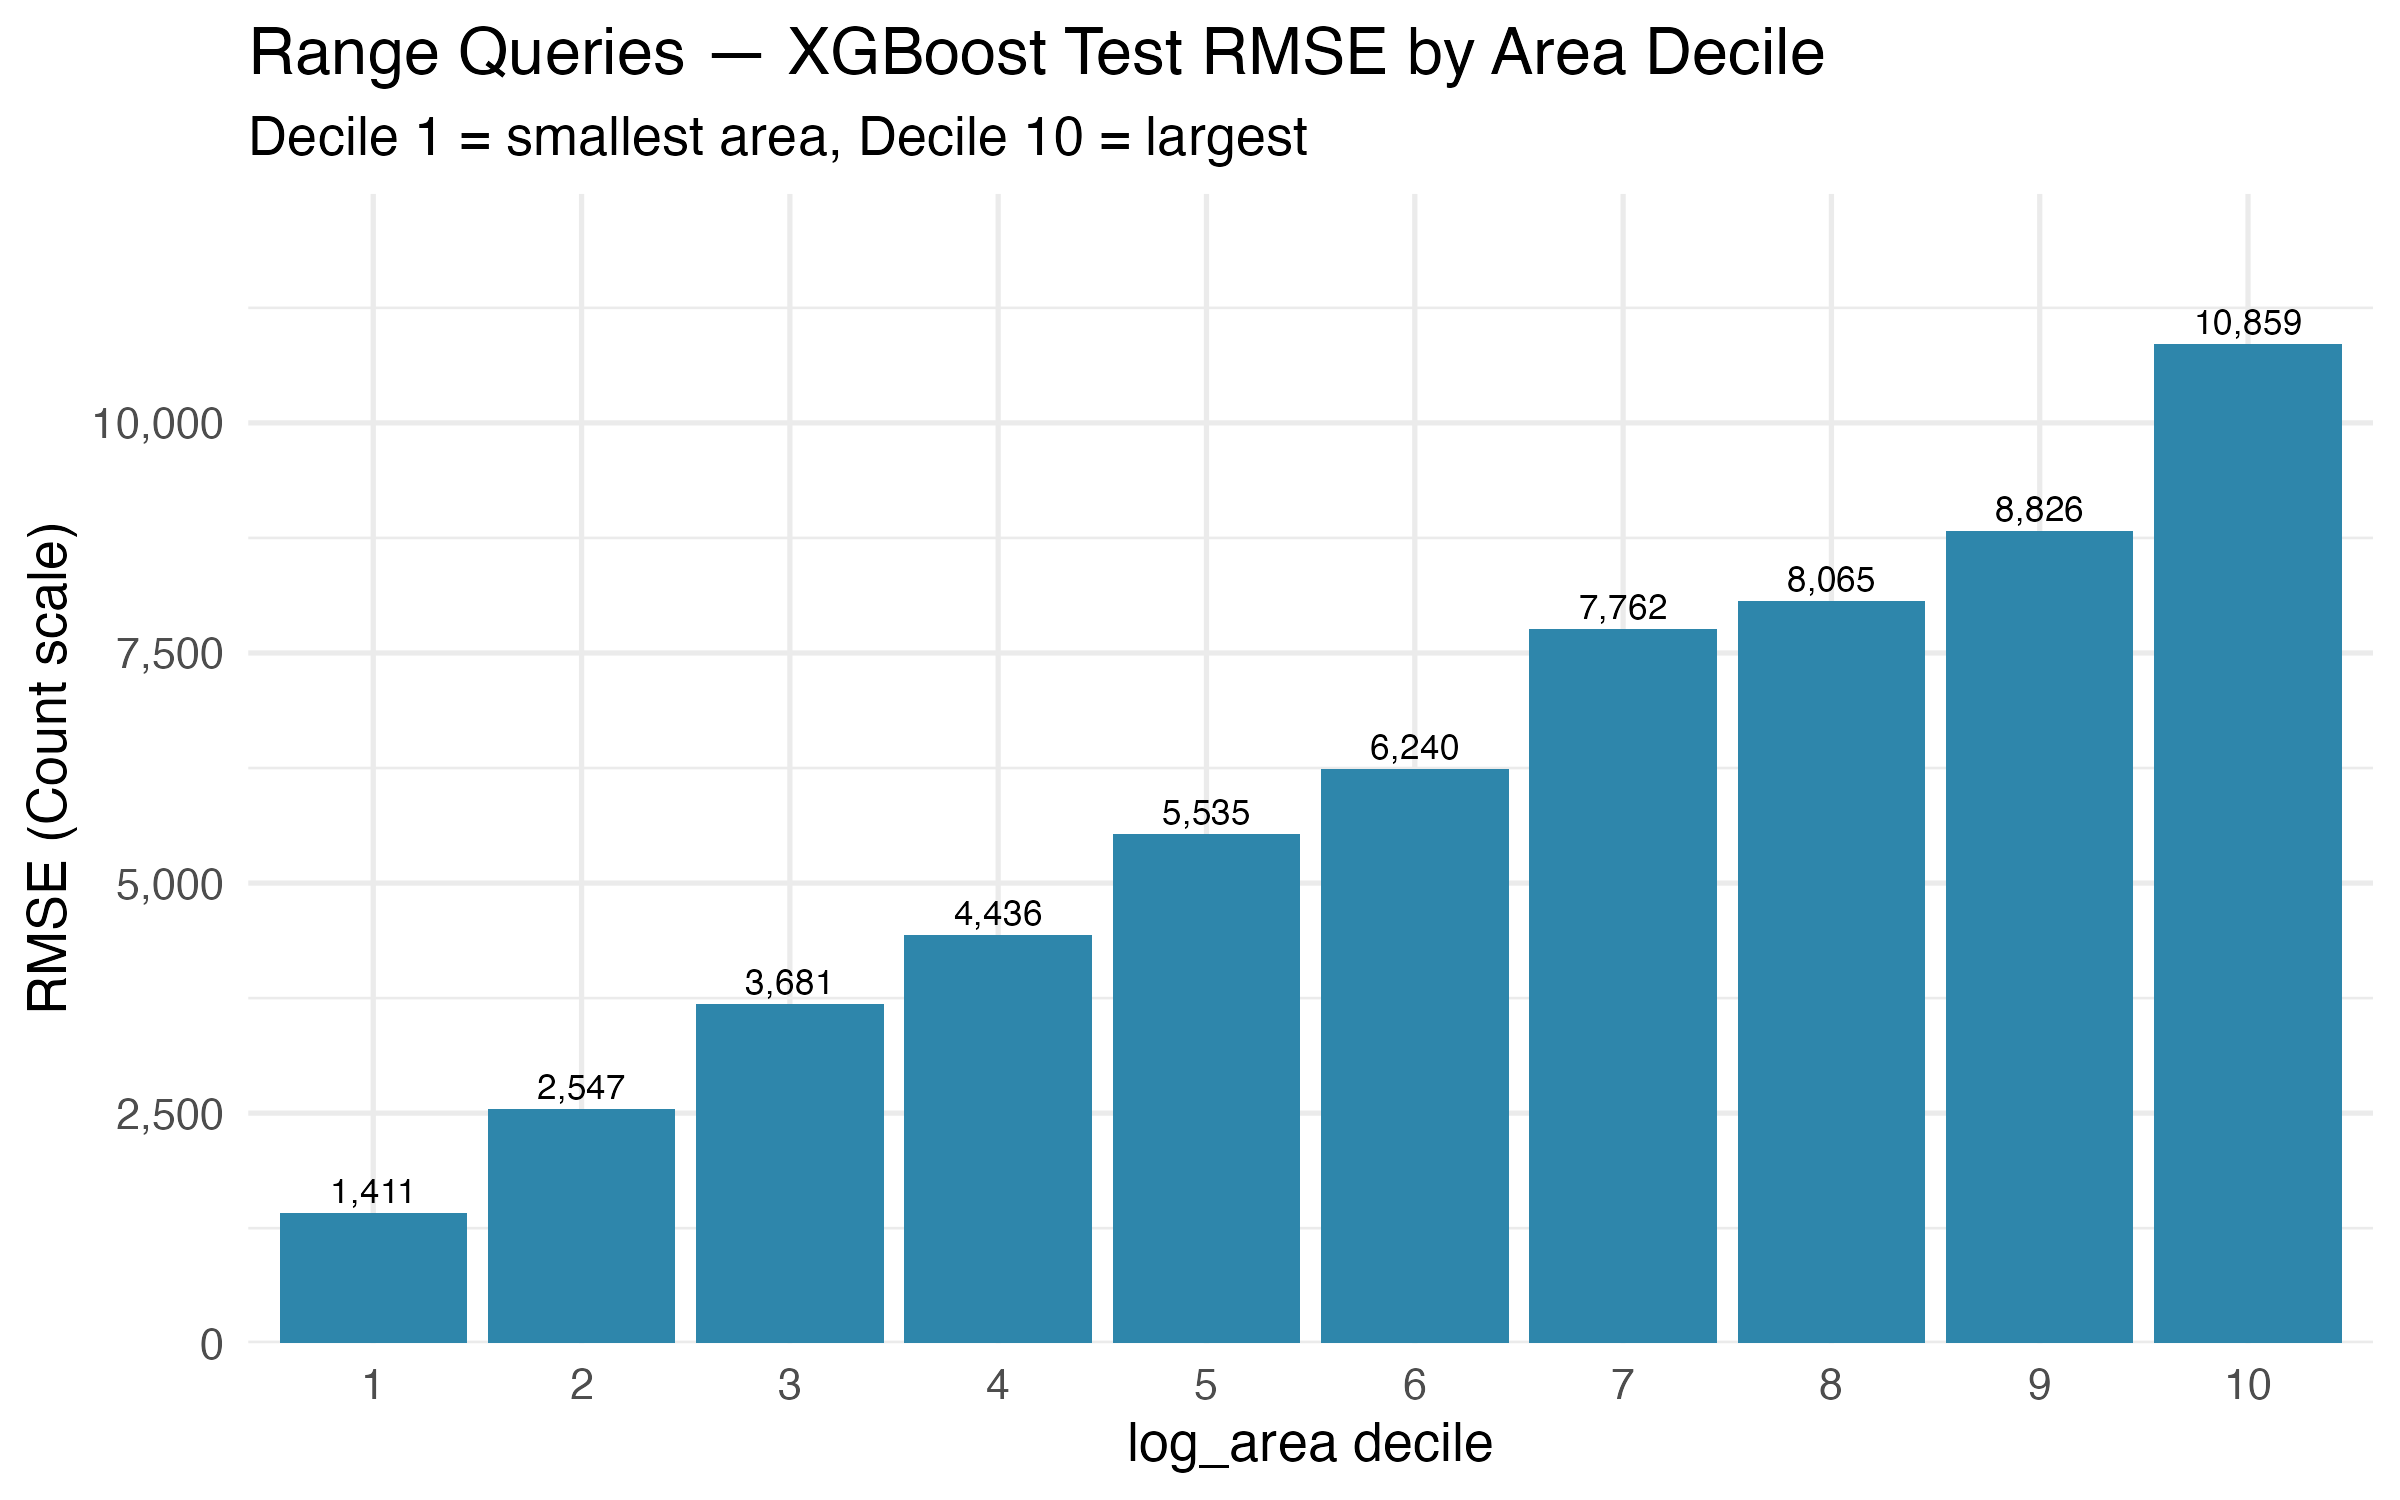
\includegraphics[width=0.95\linewidth]{figures/fig09_bias_by_quantile} \caption{Per-decile XGBoost test RMSE (Range Queries) — error rises monotonically with \texttt{log\_area}.}\label{fig:fig09}
\end{figure}

\begin{figure}[H]
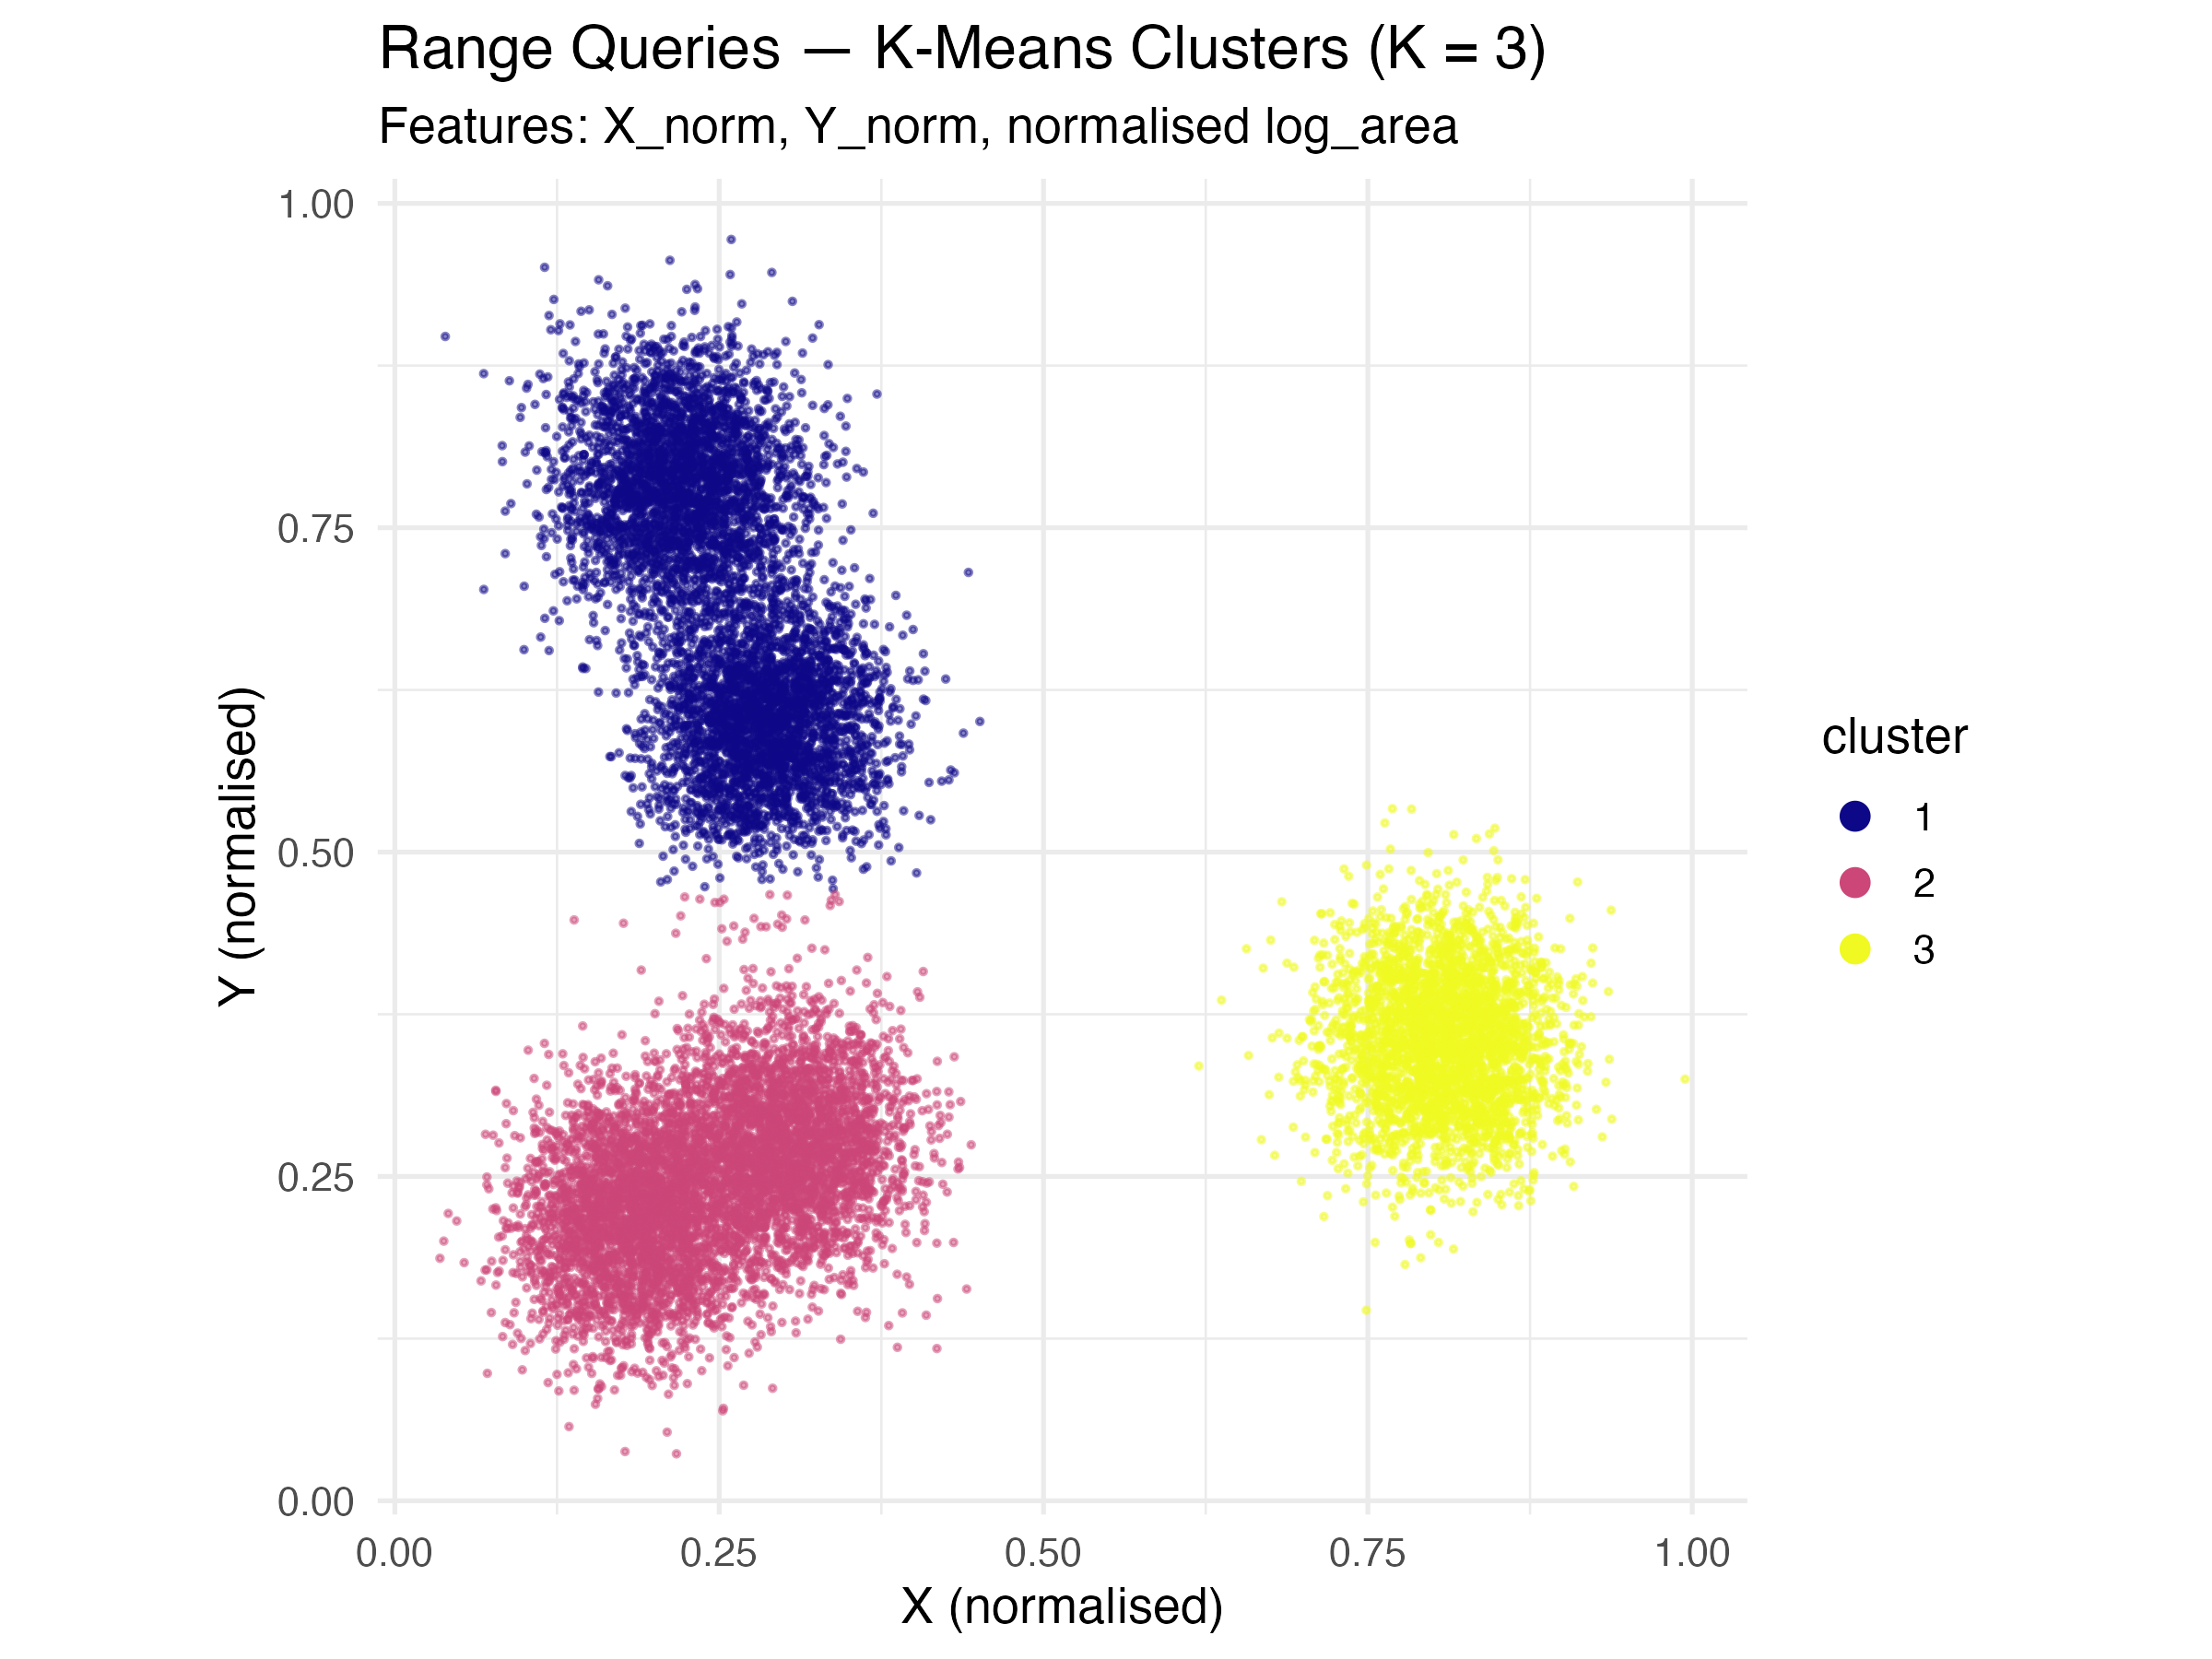
\includegraphics[width=\linewidth]{figures/fig10_clusters} \caption{K-Means clusters (K\(^*\) = 3 by silhouette) on Range Queries spatial features.}\label{fig:fig10}
\end{figure}

\section{Section 7 --- Model
Performance}\label{section-7-model-performance}

Table 1 reports test-set metrics on the original Count scale for the
four trained model families on each sub-dataset, sorted by RMSE within
dataset. Full train+test metrics are in
\texttt{results/final\_benchmark.csv}; CV grid-search results in
\texttt{results/xgb\_best\_params.csv}.

{\def\LTcaptype{none} % do not increment counter
\begin{longtable}[]{@{}
  >{\raggedright\arraybackslash}p{(\linewidth - 10\tabcolsep) * \real{0.1579}}
  >{\raggedright\arraybackslash}p{(\linewidth - 10\tabcolsep) * \real{0.1228}}
  >{\raggedright\arraybackslash}p{(\linewidth - 10\tabcolsep) * \real{0.1930}}
  >{\raggedright\arraybackslash}p{(\linewidth - 10\tabcolsep) * \real{0.1754}}
  >{\raggedright\arraybackslash}p{(\linewidth - 10\tabcolsep) * \real{0.1579}}
  >{\raggedright\arraybackslash}p{(\linewidth - 10\tabcolsep) * \real{0.1930}}@{}}
\toprule\noalign{}
\begin{minipage}[b]{\linewidth}\raggedright
Dataset
\end{minipage} & \begin{minipage}[b]{\linewidth}\raggedright
Model
\end{minipage} & \begin{minipage}[b]{\linewidth}\raggedright
Test RMSE
\end{minipage} & \begin{minipage}[b]{\linewidth}\raggedright
Test MAE
\end{minipage} & \begin{minipage}[b]{\linewidth}\raggedright
Test R²
\end{minipage} & \begin{minipage}[b]{\linewidth}\raggedright
Test MAPE
\end{minipage} \\
\midrule\noalign{}
\endhead
\bottomrule\noalign{}
\endlastfoot
Range & \textbf{XGBoost} & \textbf{6,575} & \textbf{4,411} &
\textbf{0.9982} & 10.61\% \\
Range & Random Forest & 7,801 & 4,668 & 0.9974 & 15.83\% \\
Range & KNN (K = 10) & 21,742 & 14,091 & 0.9801 & 22.24\% \\
Range & Linear & 59,655 & 40,428 & 0.8505 & 82.02\% \\
Radius & \textbf{XGBoost} & \textbf{8.52} & \textbf{5.13} &
\textbf{0.9958} & 2.31\% \\
Radius & Random Forest & 9.01 & 4.02 & 0.9953 & 1.96\% \\
Radius & KNN (K = 5) & 10.56 & 6.05 & 0.9935 & 2.74\% \\
Radius & Linear & 108.80 & 83.21 & 0.3151 & 35.50\% \\
\end{longtable}
}

\emph{Table 1.} Test-set performance on the held-out 20\% partition
(seed = 42). Best model per dataset in \textbf{bold}.

\textbf{Baseline comparison.} Against the linear baseline, XGBoost
reduces Range test RMSE by \textbf{88.9\%} (59,655 → 6,575) and Radius
test RMSE by \textbf{92.2\%} (108.80 → 8.52). The Linear R² of 0.315 on
Radius underscores why tree-based methods are essential: the radius
variable \texttt{R} has near-zero variance (SD ≈ 0.003), so any linear
function in \texttt{R} is effectively constant, and the linear model is
forced to rely on weakly-correlated spatial features.

\textbf{Why XGBoost wins.} Feature-importance analysis (fig07) shows
\texttt{log\_area} dominates with Gain = 0.63 on Range, confirming the
EDA correlation finding (Spearman ρ = 0.95 between \texttt{area} and
\texttt{Count}). Tree ensembles also capture the non-linear interaction
between query size and spatial position --- \texttt{Y\_norm} ranks first
by Random Forest \%IncMSE (importance = 144.6, vs \texttt{log\_area} =
50.9), exposing strong north--south crime-density structure that linear
correlation does not surface. XGBoost gains a further 16\% RMSE
reduction over Random Forest on Range (6,575 vs 7,801) by combining
boosting with depth-8 trees and 5-fold CV regularisation.

\textbf{Improvement summary.} XGBoost's R² of 0.998 on Range approaches
a perfect fit; the remaining absolute error is concentrated in the
highest area decile (§6, fig09). On Radius, MAE of 5.13 against a mean
Count of 265 represents ≈ 2\% relative error --- a tight fit despite the
much smaller training sample (8,000 rows). Both XGBoost models hit the
\texttt{nrounds} cap during CV, so further improvement is plausible with
extended boosting.

\section{Section 8 --- Conclusion}\label{section-8-conclusion}

\subsection{8.1 Positive Results}\label{positive-results}

XGBoost is highly effective at spatial-query selectivity estimation on
this benchmark: a Range test R² of 0.998 (RMSE = 6,575 records against a
mean Count of 159,000) and a Radius test R² of 0.996 (RMSE = 8.52
against a mean Count of 265). Against the Linear baseline, XGBoost
reduces test RMSE by 88.9\% on Range and 92.2\% on Radius. Tree-based
ensembles (XGBoost \textgreater{} Random Forest \textgreater{} KNN)
dominate the leaderboard on both sub-datasets, validating the EDA
hypothesis that the relationship between query geometry and result size
is strongly non-linear. Feature engineering --- particularly
\texttt{log\_area} and the \texttt{area\ ×\ dist\_centroid} interaction
--- was decisive: \texttt{log\_area} alone accounts for Gain = 0.63 of
the XGBoost split-improvement signal.

\subsection{8.2 Negative Results and
Caveats}\label{negative-results-and-caveats}

The Linear model fails on Radius (R² = 0.315) because the \texttt{R}
(radius) variable has near-zero variance (SD ≈ 0.003), making any linear
function in \texttt{R} effectively constant. Spatial residual analysis
(§6, fig10) reveals \textasciitilde43\% RMSE variation across K-Means
clusters, with the highest-error cluster also carrying the highest
\texttt{boundary\_flag} prevalence --- boundary-crossing queries remain
a residual-risk segment. Both XGBoost models hit the \texttt{nrounds}
cap during cross-validation (500 for Range, 300 for Radius); CV RMSE was
still decreasing, so reported metrics are upper bounds. Tree and KNN
models cannot extrapolate beyond the training feature range;
out-of-distribution queries (extreme areas, or coordinates outside the
Chicago bounding box) carry higher prediction risk.

\subsection{8.3 Recommendations and Future
Work}\label{recommendations-and-future-work}

Three concrete extensions: (i) re-train XGBoost with \texttt{nrounds} ≥
1,500 and stricter early-stopping to close the convergence gap; (ii) fit
a boundary-aware Radius model --- possibly with a separate sub-model
conditioned on \texttt{boundary\_flag} --- to address the 99.9\%
boundary-crossing rate that makes the flag uninformative as a single
feature on Radius; (iii) benchmark a small MLP or learned-index baseline
(e.g.~MSCN, Kipf et al.~2019) to test whether deep features add value
beyond hand-engineered geometric ones at this dataset scale. The current
pipeline is reproducible, deterministic (seed = 42), and runs end-to-end
in under an hour on commodity hardware, providing a solid foundation for
these extensions.

\section{Section 9 --- Data Sources}\label{section-9-data-sources}

\textbf{Primary dataset.} UCI Machine Learning Repository, Dataset
\#493: \emph{Query Analytics Workloads Dataset} (Anagnostopoulos and
Triantafillou 2015). Direct download:
\url{https://archive.ics.uci.edu/dataset/493/query+analytics+workloads+dataset}.
License: Creative Commons Attribution 4.0 (CC BY 4.0). Access: anonymous
HTTP, no authentication required.

\textbf{Underlying data.} The synthetic queries are generated against
the \emph{City of Chicago Crimes} open dataset (Chicago Police
Department, via the Chicago Data Portal:
\url{https://data.cityofchicago.org/Public-Safety/Crimes-2001-to-Present/ijzp-q8t2}),
capped at the 5.5-million-record snapshot used to compute ground-truth
aggregates for the UCI benchmark. The raw crime records themselves are
not redistributed in this repository.

\textbf{Files used.}

{\def\LTcaptype{none} % do not increment counter
\begin{longtable}[]{@{}
  >{\raggedright\arraybackslash}p{(\linewidth - 4\tabcolsep) * \real{0.3333}}
  >{\raggedright\arraybackslash}p{(\linewidth - 4\tabcolsep) * \real{0.3333}}
  >{\raggedright\arraybackslash}p{(\linewidth - 4\tabcolsep) * \real{0.3333}}@{}}
\toprule\noalign{}
\begin{minipage}[b]{\linewidth}\raggedright
File
\end{minipage} & \begin{minipage}[b]{\linewidth}\raggedright
Rows
\end{minipage} & \begin{minipage}[b]{\linewidth}\raggedright
Notes
\end{minipage} \\
\midrule\noalign{}
\endhead
\bottomrule\noalign{}
\endlastfoot
\texttt{Range-Queries-Aggregates.csv} & 200,000 & Range queries with
\texttt{Count} and \texttt{SUM} ground truth; raw Illinois State-Plane
coordinates \\
\texttt{Radius-Queries.csv} & 50,000 & Radius queries (geometry only, no
aggregates) \\
\texttt{Radius-Queries-Count.csv} & 10,000 & Radius queries with
\texttt{Count} ground truth; pre-normalised coordinates \\
\end{longtable}
}

All three raw CSVs are committed unmodified to \texttt{data/raw/}. Five
processed CSVs (described in \texttt{README.md}) plus a
\texttt{schema\_summary.csv} and \texttt{processing\_log.json} are
exported to \texttt{data/processed/} by
\texttt{Rscript\ src/preprocess.R}. Data processing is fully
reproducible with seed = 42; 100\% row retention across all three files.

\section{Section 10 --- Source Code}\label{section-10-source-code}

\textbf{Repository.} \url{https://github.com/Rahulm0106/Query-analytics}
(public, MIT-style usage).

\textbf{Layout.}

\begin{verbatim}
Query-analytics/
├── data/{raw,processed}/        # 3 raw + 5 processed CSVs
├── src/
│   ├── preprocess.R             # Day 1: data engineering pipeline
│   ├── eda.R                    # Day 2: EDA and figure generation
│   └── modeling.R               # Day 3: feature engineering + model training
├── notebooks/
│   ├── 01_preprocessing.Rmd     # Day 1 narrative
│   ├── 02_eda.Rmd               # Day 2 narrative
│   ├── 03_modeling.Rmd          # Day 3 narrative
│   └── 04_validation.Rmd        # Day 4 narrative (this report)
├── report/{sections,figures}/   # 11 markdown sections + 10 figures (300 DPI)
├── results/                     # CV / benchmark / bias CSVs
├── models/                      # Trained model objects (Git LFS)
└── renv_setup.R                 # one-shot dependency installer
\end{verbatim}

\textbf{Dependencies.} R ≥ 4.2.0 with CRAN packages: \texttt{readr},
\texttt{dplyr}, \texttt{tidyr}, \texttt{ggplot2}, \texttt{viridis},
\texttt{gridExtra}, \texttt{scales}, \texttt{car},
\texttt{randomForest}, \texttt{xgboost}, \texttt{FNN}, \texttt{cluster},
\texttt{Metrics}. All are open-source. Run
\texttt{Rscript\ renv\_setup.R} for a one-shot install; the project
ships an \texttt{renv.lock} for fully pinned versions.

\textbf{Reproducibility.} Seed = 42 throughout. End-to-end pipeline:

\begin{Shaded}
\begin{Highlighting}[]
\ExtensionTok{Rscript}\NormalTok{ renv\_setup.R                                    }\CommentTok{\# install}
\ExtensionTok{Rscript}\NormalTok{ src/preprocess.R                                }\CommentTok{\# data}
\ExtensionTok{Rscript}\NormalTok{ src/eda.R                                       }\CommentTok{\# figures 1–6}
\ExtensionTok{Rscript} \AttributeTok{{-}e} \StringTok{\textquotesingle{}rmarkdown::render("notebooks/03\_modeling.Rmd")\textquotesingle{}}   \CommentTok{\# models + fig 7}
\ExtensionTok{Rscript} \AttributeTok{{-}e} \StringTok{\textquotesingle{}rmarkdown::render("notebooks/04\_validation.Rmd")\textquotesingle{}} \CommentTok{\# validation + figs 8–10}
\end{Highlighting}
\end{Shaded}

\textbf{Note on saved models.} Trained model objects in \texttt{models/}
are tracked via Git LFS. To avoid an LFS dependency,
\texttt{notebooks/04\_validation.Rmd} refits XGBoost from
\texttt{results/xgb\_best\_params.csv} (\textasciitilde3 minutes on
commodity hardware), so all validation deliverables can be reproduced
without \texttt{git\ lfs\ pull}.

\section{Section 11 --- Bibliography}\label{section-11-bibliography}

\emph{Chicago author--date style (AMS/AIP variant).}

Anagnostopoulos, A., and P. Triantafillou, 2015: Learning to accurately
COUNT with query-driven predictive analytics. \emph{Proc. 2015 IEEE Int.
Conf. on Big Data}, Santa Clara, CA, IEEE, 14--23,
\url{https://doi.org/10.1109/BigData.2015.7363736}.

Breiman, L., 2001: Random forests. \emph{Mach. Learn.}, \textbf{45},
5--32, \url{https://doi.org/10.1023/A:1010933404324}.

Chen, T., and C. Guestrin, 2016: XGBoost: A scalable tree boosting
system. \emph{Proc. 22nd ACM SIGKDD Int. Conf. on Knowledge Discovery
and Data Mining}, San Francisco, CA, ACM, 785--794,
\url{https://doi.org/10.1145/2939672.2939785}.

City of Chicago, 2024: Crimes --- 2001 to present. Chicago Data Portal,
accessed 4 May 2026,
\url{https://data.cityofchicago.org/Public-Safety/Crimes-2001-to-Present/ijzp-q8t2}.

Dua, D., and C. Graff, 2019: UCI Machine Learning Repository. University
of California, Irvine, accessed 4 May 2026,
\url{https://archive.ics.uci.edu/}.

Kipf, A., T. Kipf, B. Radke, V. Leis, P. Boncz, and A. Kemper, 2019:
Learned cardinalities: Estimating correlated joins with deep learning.
\emph{Proc. 9th Biennial Conf. on Innovative Data Systems Research (CIDR
'19)}, Asilomar, CA, \url{https://doi.org/10.48550/arXiv.1809.00677}.

R Core Team, 2024: \emph{R: A language and environment for statistical
computing}. R Foundation for Statistical Computing, Vienna, Austria,
\url{https://www.R-project.org/}.

Wickham, H., 2016: \emph{ggplot2: Elegant Graphics for Data Analysis}.
2nd ed.~Springer-Verlag, 260 pp.,
\url{https://doi.org/10.1007/978-3-319-24277-4}.

\end{document}
